
\documentclass[lettersize,journal]{IEEEtran}
\usepackage{amsmath,amsfonts}
% \usepackage{algorithmic}
\usepackage{array}
\usepackage[caption=false,font=normalsize,labelfont=sf,textfont=sf]{subfig}
\usepackage{textcomp}
\usepackage{stfloats}
\usepackage{url}
\usepackage{verbatim}
\usepackage{graphicx}
\usepackage{cite}
\hyphenation{op-tical net-works semi-conduc-tor IEEE-Xplore}

% Optional math commands from https://github.com/goodfeli/dlbook_notation.
%%%%% NEW MATH DEFINITIONS %%%%%

\usepackage{amsmath,amsfonts,bm}

% Mark sections of captions for referring to divisions of figures
\newcommand{\figleft}{{\em (Left)}}
\newcommand{\figcenter}{{\em (Center)}}
\newcommand{\figright}{{\em (Right)}}
\newcommand{\figtop}{{\em (Top)}}
\newcommand{\figbottom}{{\em (Bottom)}}
\newcommand{\captiona}{{\em (a)}}
\newcommand{\captionb}{{\em (b)}}
\newcommand{\captionc}{{\em (c)}}
\newcommand{\captiond}{{\em (d)}}

% Highlight a newly defined term
\newcommand{\newterm}[1]{{\bf #1}}


% Figure reference, lower-case.
\def\figref#1{figure~\ref{#1}}
% Figure reference, capital. For start of sentence
\def\Figref#1{Figure~\ref{#1}}
\def\twofigref#1#2{figures \ref{#1} and \ref{#2}}
\def\quadfigref#1#2#3#4{figures \ref{#1}, \ref{#2}, \ref{#3} and \ref{#4}}
% Section reference, lower-case.
\def\secref#1{section~\ref{#1}}
% Section reference, capital.
\def\Secref#1{Section~\ref{#1}}
% Reference to two sections.
\def\twosecrefs#1#2{sections \ref{#1} and \ref{#2}}
% Reference to three sections.
\def\secrefs#1#2#3{sections \ref{#1}, \ref{#2} and \ref{#3}}
% Reference to an equation, lower-case.
\def\eqref#1{equation~\ref{#1}}
% Reference to an equation, upper case
\def\Eqref#1{Equation~\ref{#1}}
% A raw reference to an equation---avoid using if possible
\def\plaineqref#1{\ref{#1}}
% Reference to a chapter, lower-case.
\def\chapref#1{chapter~\ref{#1}}
% Reference to an equation, upper case.
\def\Chapref#1{Chapter~\ref{#1}}
% Reference to a range of chapters
\def\rangechapref#1#2{chapters\ref{#1}--\ref{#2}}
% Reference to an algorithm, lower-case.
\def\algref#1{algorithm~\ref{#1}}
% Reference to an algorithm, upper case.
\def\Algref#1{Algorithm~\ref{#1}}
\def\twoalgref#1#2{algorithms \ref{#1} and \ref{#2}}
\def\Twoalgref#1#2{Algorithms \ref{#1} and \ref{#2}}
% Reference to a part, lower case
\def\partref#1{part~\ref{#1}}
% Reference to a part, upper case
\def\Partref#1{Part~\ref{#1}}
\def\twopartref#1#2{parts \ref{#1} and \ref{#2}}

\def\ceil#1{\lceil #1 \rceil}
\def\floor#1{\lfloor #1 \rfloor}
\def\1{\bm{1}}
\newcommand{\train}{\mathcal{D}}
\newcommand{\valid}{\mathcal{D_{\mathrm{valid}}}}
\newcommand{\test}{\mathcal{D_{\mathrm{test}}}}

\def\eps{{\epsilon}}


% Random variables
\def\reta{{\textnormal{$\eta$}}}
\def\ra{{\textnormal{a}}}
\def\rb{{\textnormal{b}}}
\def\rc{{\textnormal{c}}}
\def\rd{{\textnormal{d}}}
\def\re{{\textnormal{e}}}
\def\rf{{\textnormal{f}}}
\def\rg{{\textnormal{g}}}
\def\rh{{\textnormal{h}}}
\def\ri{{\textnormal{i}}}
\def\rj{{\textnormal{j}}}
\def\rk{{\textnormal{k}}}
\def\rl{{\textnormal{l}}}
% rm is already a command, just don't name any random variables m
\def\rn{{\textnormal{n}}}
\def\ro{{\textnormal{o}}}
\def\rp{{\textnormal{p}}}
\def\rq{{\textnormal{q}}}
\def\rr{{\textnormal{r}}}
\def\rs{{\textnormal{s}}}
\def\rt{{\textnormal{t}}}
\def\ru{{\textnormal{u}}}
\def\rv{{\textnormal{v}}}
\def\rw{{\textnormal{w}}}
\def\rx{{\textnormal{x}}}
\def\ry{{\textnormal{y}}}
\def\rz{{\textnormal{z}}}

% Random vectors
\def\rvepsilon{{\mathbf{\epsilon}}}
\def\rvtheta{{\mathbf{\theta}}}
\def\rva{{\mathbf{a}}}
\def\rvb{{\mathbf{b}}}
\def\rvc{{\mathbf{c}}}
\def\rvd{{\mathbf{d}}}
\def\rve{{\mathbf{e}}}
\def\rvf{{\mathbf{f}}}
\def\rvg{{\mathbf{g}}}
\def\rvh{{\mathbf{h}}}
\def\rvu{{\mathbf{i}}}
\def\rvj{{\mathbf{j}}}
\def\rvk{{\mathbf{k}}}
\def\rvl{{\mathbf{l}}}
\def\rvm{{\mathbf{m}}}
\def\rvn{{\mathbf{n}}}
\def\rvo{{\mathbf{o}}}
\def\rvp{{\mathbf{p}}}
\def\rvq{{\mathbf{q}}}
\def\rvr{{\mathbf{r}}}
\def\rvs{{\mathbf{s}}}
\def\rvt{{\mathbf{t}}}
\def\rvu{{\mathbf{u}}}
\def\rvv{{\mathbf{v}}}
\def\rvw{{\mathbf{w}}}
\def\rvx{{\mathbf{x}}}
\def\rvy{{\mathbf{y}}}
\def\rvz{{\mathbf{z}}}

% Elements of random vectors
\def\erva{{\textnormal{a}}}
\def\ervb{{\textnormal{b}}}
\def\ervc{{\textnormal{c}}}
\def\ervd{{\textnormal{d}}}
\def\erve{{\textnormal{e}}}
\def\ervf{{\textnormal{f}}}
\def\ervg{{\textnormal{g}}}
\def\ervh{{\textnormal{h}}}
\def\ervi{{\textnormal{i}}}
\def\ervj{{\textnormal{j}}}
\def\ervk{{\textnormal{k}}}
\def\ervl{{\textnormal{l}}}
\def\ervm{{\textnormal{m}}}
\def\ervn{{\textnormal{n}}}
\def\ervo{{\textnormal{o}}}
\def\ervp{{\textnormal{p}}}
\def\ervq{{\textnormal{q}}}
\def\ervr{{\textnormal{r}}}
\def\ervs{{\textnormal{s}}}
\def\ervt{{\textnormal{t}}}
\def\ervu{{\textnormal{u}}}
\def\ervv{{\textnormal{v}}}
\def\ervw{{\textnormal{w}}}
\def\ervx{{\textnormal{x}}}
\def\ervy{{\textnormal{y}}}
\def\ervz{{\textnormal{z}}}

% Random matrices
\def\rmA{{\mathbf{A}}}
\def\rmB{{\mathbf{B}}}
\def\rmC{{\mathbf{C}}}
\def\rmD{{\mathbf{D}}}
\def\rmE{{\mathbf{E}}}
\def\rmF{{\mathbf{F}}}
\def\rmG{{\mathbf{G}}}
\def\rmH{{\mathbf{H}}}
\def\rmI{{\mathbf{I}}}
\def\rmJ{{\mathbf{J}}}
\def\rmK{{\mathbf{K}}}
\def\rmL{{\mathbf{L}}}
\def\rmM{{\mathbf{M}}}
\def\rmN{{\mathbf{N}}}
\def\rmO{{\mathbf{O}}}
\def\rmP{{\mathbf{P}}}
\def\rmQ{{\mathbf{Q}}}
\def\rmR{{\mathbf{R}}}
\def\rmS{{\mathbf{S}}}
\def\rmT{{\mathbf{T}}}
\def\rmU{{\mathbf{U}}}
\def\rmV{{\mathbf{V}}}
\def\rmW{{\mathbf{W}}}
\def\rmX{{\mathbf{X}}}
\def\rmY{{\mathbf{Y}}}
\def\rmZ{{\mathbf{Z}}}

% Elements of random matrices
\def\ermA{{\textnormal{A}}}
\def\ermB{{\textnormal{B}}}
\def\ermC{{\textnormal{C}}}
\def\ermD{{\textnormal{D}}}
\def\ermE{{\textnormal{E}}}
\def\ermF{{\textnormal{F}}}
\def\ermG{{\textnormal{G}}}
\def\ermH{{\textnormal{H}}}
\def\ermI{{\textnormal{I}}}
\def\ermJ{{\textnormal{J}}}
\def\ermK{{\textnormal{K}}}
\def\ermL{{\textnormal{L}}}
\def\ermM{{\textnormal{M}}}
\def\ermN{{\textnormal{N}}}
\def\ermO{{\textnormal{O}}}
\def\ermP{{\textnormal{P}}}
\def\ermQ{{\textnormal{Q}}}
\def\ermR{{\textnormal{R}}}
\def\ermS{{\textnormal{S}}}
\def\ermT{{\textnormal{T}}}
\def\ermU{{\textnormal{U}}}
\def\ermV{{\textnormal{V}}}
\def\ermW{{\textnormal{W}}}
\def\ermX{{\textnormal{X}}}
\def\ermY{{\textnormal{Y}}}
\def\ermZ{{\textnormal{Z}}}

% Vectors
\def\vzero{{\bm{0}}}
\def\vone{{\bm{1}}}
\def\vmu{{\bm{\mu}}}
\def\vtheta{{\bm{\theta}}}
\def\va{{\bm{a}}}
\def\vb{{\bm{b}}}
\def\vc{{\bm{c}}}
\def\vd{{\bm{d}}}
\def\ve{{\bm{e}}}
\def\vf{{\bm{f}}}
\def\vg{{\bm{g}}}
\def\vh{{\bm{h}}}
\def\vi{{\bm{i}}}
\def\vj{{\bm{j}}}
\def\vk{{\bm{k}}}
\def\vl{{\bm{l}}}
\def\vm{{\bm{m}}}
\def\vn{{\bm{n}}}
\def\vo{{\bm{o}}}
\def\vp{{\bm{p}}}
\def\vq{{\bm{q}}}
\def\vr{{\bm{r}}}
\def\vs{{\bm{s}}}
\def\vt{{\bm{t}}}
\def\vu{{\bm{u}}}
\def\vv{{\bm{v}}}
\def\vw{{\bm{w}}}
\def\vx{{\bm{x}}}
\def\vy{{\bm{y}}}
\def\vz{{\bm{z}}}

% Elements of vectors
\def\evalpha{{\alpha}}
\def\evbeta{{\beta}}
\def\evepsilon{{\epsilon}}
\def\evlambda{{\lambda}}
\def\evomega{{\omega}}
\def\evmu{{\mu}}
\def\evpsi{{\psi}}
\def\evsigma{{\sigma}}
\def\evtheta{{\theta}}
\def\eva{{a}}
\def\evb{{b}}
\def\evc{{c}}
\def\evd{{d}}
\def\eve{{e}}
\def\evf{{f}}
\def\evg{{g}}
\def\evh{{h}}
\def\evi{{i}}
\def\evj{{j}}
\def\evk{{k}}
\def\evl{{l}}
\def\evm{{m}}
\def\evn{{n}}
\def\evo{{o}}
\def\evp{{p}}
\def\evq{{q}}
\def\evr{{r}}
\def\evs{{s}}
\def\evt{{t}}
\def\evu{{u}}
\def\evv{{v}}
\def\evw{{w}}
\def\evx{{x}}
\def\evy{{y}}
\def\evz{{z}}

% Matrix
\def\mA{{\bm{A}}}
\def\mB{{\bm{B}}}
\def\mC{{\bm{C}}}
\def\mD{{\bm{D}}}
\def\mE{{\bm{E}}}
\def\mF{{\bm{F}}}
\def\mG{{\bm{G}}}
\def\mH{{\bm{H}}}
\def\mI{{\bm{I}}}
\def\mJ{{\bm{J}}}
\def\mK{{\bm{K}}}
\def\mL{{\bm{L}}}
\def\mM{{\bm{M}}}
\def\mN{{\bm{N}}}
\def\mO{{\bm{O}}}
\def\mP{{\bm{P}}}
\def\mQ{{\bm{Q}}}
\def\mR{{\bm{R}}}
\def\mS{{\bm{S}}}
\def\mT{{\bm{T}}}
\def\mU{{\bm{U}}}
\def\mV{{\bm{V}}}
\def\mW{{\bm{W}}}
\def\mX{{\bm{X}}}
\def\mY{{\bm{Y}}}
\def\mZ{{\bm{Z}}}
\def\mBeta{{\bm{\beta}}}
\def\mPhi{{\bm{\Phi}}}
\def\mLambda{{\bm{\Lambda}}}
\def\mSigma{{\bm{\Sigma}}}

% Tensor
\DeclareMathAlphabet{\mathsfit}{\encodingdefault}{\sfdefault}{m}{sl}
\SetMathAlphabet{\mathsfit}{bold}{\encodingdefault}{\sfdefault}{bx}{n}
\newcommand{\tens}[1]{\bm{\mathsfit{#1}}}
\def\tA{{\tens{A}}}
\def\tB{{\tens{B}}}
\def\tC{{\tens{C}}}
\def\tD{{\tens{D}}}
\def\tE{{\tens{E}}}
\def\tF{{\tens{F}}}
\def\tG{{\tens{G}}}
\def\tH{{\tens{H}}}
\def\tI{{\tens{I}}}
\def\tJ{{\tens{J}}}
\def\tK{{\tens{K}}}
\def\tL{{\tens{L}}}
\def\tM{{\tens{M}}}
\def\tN{{\tens{N}}}
\def\tO{{\tens{O}}}
\def\tP{{\tens{P}}}
\def\tQ{{\tens{Q}}}
\def\tR{{\tens{R}}}
\def\tS{{\tens{S}}}
\def\tT{{\tens{T}}}
\def\tU{{\tens{U}}}
\def\tV{{\tens{V}}}
\def\tW{{\tens{W}}}
\def\tX{{\tens{X}}}
\def\tY{{\tens{Y}}}
\def\tZ{{\tens{Z}}}


% Graph
\def\gA{{\mathcal{A}}}
\def\gB{{\mathcal{B}}}
\def\gC{{\mathcal{C}}}
\def\gD{{\mathcal{D}}}
\def\gE{{\mathcal{E}}}
\def\gF{{\mathcal{F}}}
\def\gG{{\mathcal{G}}}
\def\gH{{\mathcal{H}}}
\def\gI{{\mathcal{I}}}
\def\gJ{{\mathcal{J}}}
\def\gK{{\mathcal{K}}}
\def\gL{{\mathcal{L}}}
\def\gM{{\mathcal{M}}}
\def\gN{{\mathcal{N}}}
\def\gO{{\mathcal{O}}}
\def\gP{{\mathcal{P}}}
\def\gQ{{\mathcal{Q}}}
\def\gR{{\mathcal{R}}}
\def\gS{{\mathcal{S}}}
\def\gT{{\mathcal{T}}}
\def\gU{{\mathcal{U}}}
\def\gV{{\mathcal{V}}}
\def\gW{{\mathcal{W}}}
\def\gX{{\mathcal{X}}}
\def\gY{{\mathcal{Y}}}
\def\gZ{{\mathcal{Z}}}

% Sets
\def\sA{{\mathbb{A}}}
\def\sB{{\mathbb{B}}}
\def\sC{{\mathbb{C}}}
\def\sD{{\mathbb{D}}}
% Don't use a set called E, because this would be the same as our symbol
% for expectation.
\def\sF{{\mathbb{F}}}
\def\sG{{\mathbb{G}}}
\def\sH{{\mathbb{H}}}
\def\sI{{\mathbb{I}}}
\def\sJ{{\mathbb{J}}}
\def\sK{{\mathbb{K}}}
\def\sL{{\mathbb{L}}}
\def\sM{{\mathbb{M}}}
\def\sN{{\mathbb{N}}}
\def\sO{{\mathbb{O}}}
\def\sP{{\mathbb{P}}}
\def\sQ{{\mathbb{Q}}}
\def\sR{{\mathbb{R}}}
\def\sS{{\mathbb{S}}}
\def\sT{{\mathbb{T}}}
\def\sU{{\mathbb{U}}}
\def\sV{{\mathbb{V}}}
\def\sW{{\mathbb{W}}}
\def\sX{{\mathbb{X}}}
\def\sY{{\mathbb{Y}}}
\def\sZ{{\mathbb{Z}}}

% Entries of a matrix
\def\emLambda{{\Lambda}}
\def\emA{{A}}
\def\emB{{B}}
\def\emC{{C}}
\def\emD{{D}}
\def\emE{{E}}
\def\emF{{F}}
\def\emG{{G}}
\def\emH{{H}}
\def\emI{{I}}
\def\emJ{{J}}
\def\emK{{K}}
\def\emL{{L}}
\def\emM{{M}}
\def\emN{{N}}
\def\emO{{O}}
\def\emP{{P}}
\def\emQ{{Q}}
\def\emR{{R}}
\def\emS{{S}}
\def\emT{{T}}
\def\emU{{U}}
\def\emV{{V}}
\def\emW{{W}}
\def\emX{{X}}
\def\emY{{Y}}
\def\emZ{{Z}}
\def\emSigma{{\Sigma}}

% entries of a tensor
% Same font as tensor, without \bm wrapper
\newcommand{\etens}[1]{\mathsfit{#1}}
\def\etLambda{{\etens{\Lambda}}}
\def\etA{{\etens{A}}}
\def\etB{{\etens{B}}}
\def\etC{{\etens{C}}}
\def\etD{{\etens{D}}}
\def\etE{{\etens{E}}}
\def\etF{{\etens{F}}}
\def\etG{{\etens{G}}}
\def\etH{{\etens{H}}}
\def\etI{{\etens{I}}}
\def\etJ{{\etens{J}}}
\def\etK{{\etens{K}}}
\def\etL{{\etens{L}}}
\def\etM{{\etens{M}}}
\def\etN{{\etens{N}}}
\def\etO{{\etens{O}}}
\def\etP{{\etens{P}}}
\def\etQ{{\etens{Q}}}
\def\etR{{\etens{R}}}
\def\etS{{\etens{S}}}
\def\etT{{\etens{T}}}
\def\etU{{\etens{U}}}
\def\etV{{\etens{V}}}
\def\etW{{\etens{W}}}
\def\etX{{\etens{X}}}
\def\etY{{\etens{Y}}}
\def\etZ{{\etens{Z}}}

% The true underlying data generating distribution
\newcommand{\pdata}{p_{\rm{data}}}
% The empirical distribution defined by the training set
\newcommand{\ptrain}{\hat{p}_{\rm{data}}}
\newcommand{\Ptrain}{\hat{P}_{\rm{data}}}
% The model distribution
\newcommand{\pmodel}{p_{\rm{model}}}
\newcommand{\Pmodel}{P_{\rm{model}}}
\newcommand{\ptildemodel}{\tilde{p}_{\rm{model}}}
% Stochastic autoencoder distributions
\newcommand{\pencode}{p_{\rm{encoder}}}
\newcommand{\pdecode}{p_{\rm{decoder}}}
\newcommand{\precons}{p_{\rm{reconstruct}}}

\newcommand{\laplace}{\mathrm{Laplace}} % Laplace distribution

\newcommand{\E}{\mathbb{E}}
\newcommand{\Ls}{\mathcal{L}}
\newcommand{\R}{\mathbb{R}}
\newcommand{\emp}{\tilde{p}}
\newcommand{\lr}{\alpha}
\newcommand{\reg}{\lambda}
\newcommand{\rect}{\mathrm{rectifier}}
\newcommand{\softmax}{\mathrm{softmax}}
\newcommand{\sigmoid}{\sigma}
\newcommand{\softplus}{\zeta}
\newcommand{\KL}{D_{\mathrm{KL}}}
\newcommand{\Var}{\mathrm{Var}}
\newcommand{\standarderror}{\mathrm{SE}}
\newcommand{\Cov}{\mathrm{Cov}}
% Wolfram Mathworld says $L^2$ is for function spaces and $\ell^2$ is for vectors
% But then they seem to use $L^2$ for vectors throughout the site, and so does
% wikipedia.
\newcommand{\normlzero}{L^0}
\newcommand{\normlone}{L^1}
\newcommand{\normltwo}{L^2}
\newcommand{\normlp}{L^p}
\newcommand{\normmax}{L^\infty}

\newcommand{\parents}{Pa} % See usage in notation.tex. Chosen to match Daphne's book.

\DeclareMathOperator*{\argmax}{arg\,max}
\DeclareMathOperator*{\argmin}{arg\,min}

\DeclareMathOperator{\sign}{sign}
\DeclareMathOperator{\Tr}{Tr}
\let\ab\allowbreak


\usepackage{hyperref}
\usepackage{wrapfig}  
\graphicspath{ {./images/} }

% Required packages
\usepackage{algorithm}
\usepackage{algpseudocode}
\usepackage{amsmath} % for math environments
\usepackage{xcolor, colortbl}  % for color
\usepackage{tcolorbox} % for colored boxes
% Define custom colors
\definecolor{myblue}{RGB}{44, 130, 201}
\definecolor{mygreen}{RGB}{34, 177, 76}
\definecolor{myred}{RGB}{237, 28, 36}
\definecolor{myorange}{RGB}{255, 127, 39}

%for table
\usepackage{tabularx}
\usepackage{booktabs}
\usepackage{pifont}
\usepackage{adjustbox}
\usepackage{multirow}

%for bar plot
\usepackage{pgfplots}
\usepackage{tikz}
\pgfplotsset{compat=1.17}

% Define custom commands
\newcommand{\todo}[1]{\textcolor{red}{[#1]}}
\newcommand{\todoa}[1]{\textcolor{blue}{[#1]}}
\newcommand{\tohl}[1]{\textcolor{cyan}{[#1]}}

\newtheorem{assumption}{Assumption}
\newtheorem{theorem}{Theorem}
\newtheorem{lemma}{Lemma}
\newtheorem{proof}{Proof}
\newtheorem{definition}{Definition}

\title{\textsf{ProtoGen}: Federated Privacy-Preserving Prototype Learning via Feature Generation in Heterogeneous Environments}

\author{Sujit~Chowdhury, Aritra Bhaduri, Raju Halder% <-this % stops a space
\IEEEcompsocitemizethanks{\IEEEcompsocthanksitem Sujit Chowdhury, Aritra Bhaduri, Raju Halder are with the Department
of Computer Science and Engineering, Indian Institute of Technology Patna, 
India, 801106.\protect\\
% note need leading \protect in front of \\ to get a newline within \thanks as
% \\ is fragile and will error, could use \hfil\break instead.
E-mail: \{sujit\_2021cs35, aritra\_2101ai40, halder\}@iitp.ac.in}
% \And
% Ji Q. Ren \& Yevgeny LeNet \\
% Department of Computational Neuroscience \\
% University of the Witwatersrand \\
% Joburg, South Africa \\
% \texttt{\{robot,net\}@wits.ac.za} \\
% \AND
% Coauthor \\
% Affiliation \\
% Address \\
% \texttt{email}
}

% The \author macro works with any number of authors. There are two commands
% used to separate the names and addresses of multiple authors: \And and \AND.
%
% Using \And between authors leaves it to \LaTeX{} to determine where to break
% the lines. Using \AND forces a linebreak at that point. So, if \LaTeX{}
% puts 3 of 4 authors names on the first line, and the last on the second
% line, try using \AND instead of \And before the third author name.

\newcommand{\fix}{\marginpar{FIX}}
\newcommand{\new}{\marginpar{NEW}}

% \iclrfinalcopy % Uncomment for camera-ready version, but NOT for submission.
\begin{document}


\maketitle

\begin{abstract}
	Federated Learning (FL) enables collaborative model training across decentralized clients without sharing raw data. However, its performance declines when faced with heterogeneous data distributions across participating clients. To address this, existing FL frameworks often share not only locally trained model parameters but also additional client-specific information, which increases communication overhead and heightens privacy risks. In this paper, we propose \textsf{ProtoGen}, a novel FL framework that leverages privacy-preserving feature generation and prototype-based representation alignment to address these challenges in a unified and communication-efficient manner. Specifically, the framework introduces a Privacy-Preserving Generative Module (\emph{PPGM}) that enables each client to train a lightweight generative model on differentially private feature embeddings and share its trained parameters with the server, eliminating the need to expose raw data or intermediate representations, thereby reducing communication cost and enhancing data privacy. To construct global class-wise prototypes, \textsf{ProtoGen} incorporates a novel server-side prototype construction mechanism that aggregates synthesized class-wise features using these shared generative model parameters for all clients. This design allows the clients to perform local feature alignment through the constructed global prototypes and to fine-tune the classifier layer via synthesizing underrepresented class features utilizing \emph{PPGM}, enabling effective local model training across heterogeneous clients and substantially mitigating data distribution skew. Our experiments on benchmark datasets—MNIST, CIFAR-10, and CIFAR-100—show that \textsf{ProtoGen} consistently improves model convergence and test accuracy by an average of 4.76\% over state-of-the-art FL methods, while significantly reducing communication overhead and preserving privacy.
\end{abstract}


\begin{IEEEkeywords}
Federated Learning, \and Prototype Learning, \and Generative Model, \and Privacy Preserving, \and Data Heterogeneity
\end{IEEEkeywords}

\section{Introduction}

Federated Learning (FL) has gained prominence as an effective approach for collaboratively training machine learning models across decentralized datasets, ensuring data privacy by eliminating the need to share raw data between clients~\cite{mcmahan2017communication}. Despite its potential, FL performance tends to degrade significantly when data distributions across clients are highly heterogeneous or non-independent and identically distributed (non-IID)~\cite{zhao2018federated}. The heterogeneity in FL appears in various forms, such as label skewness, feature skewness, quantity skewness, which pose significant challenges for model training and generalization.
\todoa{To combat with the effect of heterogeneity, recent research has explored various strategies, including variance reduction \cite{acar2021federated, karimireddy2020scaffold}, adaptive aggregation \cite{hsu2019measuring, fedadam, fednova, reddi2021adaptive, chen2023elastic, Chen_2023_CVPR}, feature distillation \cite{yang2023fedfed}, and representation learning \cite{zhang2020federated, tan2022federated, liu2024federated}. Notably, most of the proposed solutions under these strategies involve sharing  additional information between clients and server such as control variates, client features, and classifier characteristics, which leads to increased communication costs and heightened risks of privacy breaches \cite{nasr2019comprehensive,melis2019exploiting, wang2019beyond}. Whereas, prototype-based solution \cite{tan2022fedproto} has emerged as a promising alternative, since it shares only class-wise feature prototypes instead of full model parameters, thereby reducing communication overhead and exposure of sensitive information. However, as like others, the approach considers only a subset of clients - assuming that in practice few clients may not be available for training due to various issues like connectivity, power constraints, or computational limitations. As a result, the aggregated prototypes are biased toward the data distribution of active clients, neglecting information from inactive ones. This problem is further exacerbated under heterogeneous and imbalanced data distributions, where the absence of minority-class clients disproportionately skews the global representation and degrades generalization in subsequent rounds.}

%\todoa{These emphasize a clear need for a holistic approach that construct unbiased global representations under partial participation without sacrificing privacy or communication efficiency. Motivated by these limitations, we investigate the following research questions (RQs):}

\todoa{These observations point to a persistent research gap. FL systems need mechanisms that (i) construct global representations that remain \emph{unbiased and temporally consistent} under partial participation, (ii) preserve privacy beyond raw data protection by preventing leakage of hidden features or gradients, and (iii) achieve these goals in a communication-efficient manner suitable for resource-constrained environments. Existing solutions typically address one of these aspects in isolation but compromise others. For instance, variance-reduction and adaptive aggregation approaches may improve stability but at high communication cost. Distillation-based methods enhance alignment but heighten privacy risks. Prototype learning improves efficiency but collapses under partial client participation. Thus, there is a clear need for a holistic framework that integrates unbiased prototype construction with privacy guarantees and communication efficiency. Motivated by these gaps, we focus on the following research questions (RQs):}

%\textit{RQ1: How can a global representation in FL be constructed in a way that remains unbiased and temporally consistent, even when only a subset of clients participate in each round?}
\textit{RQ1: How can a global representation in FL remain unbiased and temporally consistent under partial client participation?}
%How can unbiased and temporally stable global prototypes be constructed under partial client participation, while incorporating knowledge from inactive clients efficiently across rounds?

\textit{RQ2: How can local training be decoupled from server-side aggregation in a way that preserves privacy yet avoids the trade-off of degraded training performance?}

\todoa{\noindent Addressing these questions requires rethinking both client-side and server-side operations. Locally, models must align with global representations without leaking private information; globally, prototypes must integrate knowledge from both active and inactive clients to avoid bias.} 
 
%These emphasize a clear need for a holistic approach that reduces communication cost while enhances model performance as well as data privacy. To address this, we revisit the foundational strategies for mitigating the impact of data heterogeneity in federated systems, which led us to explore the following research questions (RQs).

%\textit{RQ1: How can a global representation in FL be constructed without being biased due to partial client participation?}In real-world applications, it is impractical to assume that all clients will be available for training at all times due to connectivity issues, power constraints, and computational limitations. As a result, existing FL algorithms train local models using only a partial set of clients in each round, leading to biased global representations that fail to capture the full data distribution. This becomes more severe in highly heterogeneous settings where the absence of certain clients skews the global representation, which eventually causes poor generalization across the participating clients in the next round. A potential solution is to construct a more comprehensive global representation by leveraging information from all clients, including those not active in a given round. To achieve this, we introduce a privacy preserving feature generation module, where each client trains a generative model to synthesize class-specific features instead of sharing raw features or model updates. By aggregating the generated features from all available generative models, the server constructs a robust global feature representation, ensuring consistency even when a subset of clients participates in every round. Unlike existing approaches that rely solely on currently available client data, our approach leverages historical feature generator parameters from previous rounds when a client is unavailable. By incorporating both current and past client representations, our method ensures a more consistent, generalized, and robust global model, even under partial client participation.
%\textit{RQ2: How can privacy be preserved while constructing the global representation?}Existing FL approaches often struggle to balance privacy protection with model performance, especially when dealing with heterogeneous data distributions across clients. Conventional methods which transmit model parameters, gradients, or extracted features are highly vulnerable to inference attacks, such as membership inference, feature reconstruction, and model inversion \cite{nasr2019comprehensive,melis2019exploiting, wang2019beyond}. Even when raw data is not shared, adversaries can exploit hidden feature representations or gradients to infer sensitive client information. Training a privacy-preserving generative module at each client and transmitting only the feature generator parameters of the trained generative model ensures that no direct feature representations are exposed. This approach enhances privacy by preventing the reconstruction of sensitive client information while still allowing the server to synthesize meaningful feature representations.
%\textit{RQ3: How to mitigate communication overhead for a communication-constraint FL environment?} Communication overhead is a critical challenge in FL, as it significantly affects overall training efficiency. In communication-constrained environments, the cost of transmitting data between clients and the central server can become a bottleneck, slowing down the entire training process. To address this, communication costs can be reduced by carefully selecting and compressing the information exchanged between clients and the server. One promising direction is to reduce the need for full model updates by sharing only compact, informative representations, such as feature-level representations or learned embeddings.


\todoa{In response to the above research questions, we propose \textsf{ProtoGen} (Federated Privacy-Preserving \textbf{Proto}type Learning via Feature \textbf{Gen}eration in Heterogeneous Environments), a novel FL framework that systematically eliminates prototype bias under partial participation while simultaneously enhancing privacy and reducing communication cost. At its core \textsf{ProtoGen} introduces a lightweight \emph{class-wise feature generative module} at each client. This module learns to synthesize class-specific features that reflect the client’s local distribution. On the client side, the generated features are used to augment missing classes and fine-tune classifier layers, thereby mitigating classifier drift and class imbalance in non-IID settings. On the server side, \textsf{ProtoGen} utilizes the shared generator parameters to synthesize class-wise features and construct global prototypes. Crucially, the server can regenerate features not only from currently active clients but also from inactive ones using their previously shared generators, yielding prototypes that are unbiased and temporally consistent across rounds, directly addressing \textit{RQ1}. To ensure privacy without compromising model utility, \textsf{ProtoGen} \emph{decouples local learning into two phases}: Phase-1 trains the main classifier on raw data to preserve predictive performance, while Phase-2 trains the generative module on noise-perturbed data, ensuring differential privacy. Only the generator parameters are shared, substantially reducing communication cost and protecting sensitive model information. This two-phase design resolves \textit{RQ2}, as privacy is enforced without weakening the classification model. Together, these mechanisms allow \textsf{ProtoGen} to deliver robust global prototypes, privacy guarantees, and communication efficiency in one integrated framework.} 

%\todo{The main idea is to replace direct feature exchange with lightweight privacy-preserving generative models that synthesize class-wise features for both active and inactive clients, enabling the server to construct unbiased and representative global prototypes. To realize this idea, \textsf{ProtoGen} incorporates three tightly coupled design components:(1) Class-wise Prototype Construction (addresses RQ1). At the core of \textsf{ProtoGen} is a new scheme for constructing global prototypes that remain unbiased even under partial client participation. Rather than aggregating only from active clients, the server synthesizes class-specific features using generative parameters shared by all clients (active or inactive). Historical generators allow the server to recover features from previously active clients, ensuring that no round is dominated by a biased subset. This yields a more complete and representative global feature space, directly mitigating the prototype bias problem caused by partial participation and heterogeneity. (2) Privacy-Preserving Generative Module (addresses RQ2). To enable this construction without exposing sensitive client data, we introduce a \textit{Privacy-Preserving Generative Module} (PPGM). Each client trains its PPGM to learn class-conditional feature distributions, but instead of sharing raw or directly extractable features, Gaussian noise is injected into the raw data before feature extraction. This controlled perturbation prevents identifiable patterns from leaking while still preserving task-relevant information. Clients transmit only the lightweight generator parameters to the server, significantly reducing communication cost. By decoupling local model training from generator training, PPGM ensures that privacy is preserved without degrading classifier performance — overcoming the typical trade-off between privacy and utility. (3) Classifier Tuning via Synthetic Features (supports RQ1 and RQ3). Finally, the availability of class-specific generators allows clients to synthesize features for \emph{all} classes, including those absent in their local datasets. These synthetic features are used to tune classifier weights, reducing classifier drift among clients and mitigating class imbalance in non-IID environments. This mechanism ensures that clients align their decision boundaries with the federation-wide distribution, further enhancing generalization across rounds.  }
\begin{figure}
	\centering
	\begin{tabular}{ccc}
		$\beta = 0.1$ & $\beta = 0.5$ & $\beta = 0.05$ \\
		\scalebox{0.29}{
			\begin{tikzpicture}
				\begin{axis}[
					xlabel={Rounds},
					ylabel={Similiarity},
					grid=both,
					ymin=-1,
					xmin=0,
					xmax=100,
					legend style={
						at={(0.84,0.24)},
						anchor=north,
						legend cell align=left,
						legend columns=1,
						font=\scriptsize,
						draw=black, % Remove border around legend
						fill=white, % Remove background color of legend
						inner sep=3pt, % Adjust inner padding of legend box
						legend image post style={scale=0.5}, % Adjust size of legend marker
					},
					]
					\addplot[thick, color=orange] table {Tables/layer_sim/one/similarities_l_0_one_cifar_b_1.table};
					\addplot[thick, color=blue] table {Tables/layer_sim/one/similarities_l_1_one_cifar_b_1.table};
					\addplot[thick, color=magenta] table {Tables/layer_sim/one/similarities_l_2_one_cifar_b_1.table};
					
					\addlegendentry {Layer 1}
					\addlegendentry {Layer 2}
					\addlegendentry {\textbf{Classifier layer}}
					
				\end{axis}
				
			\end{tikzpicture}
		}
		&
		\scalebox{0.29}{
			\begin{tikzpicture}
				\begin{axis}[
					xlabel={Rounds},
					ylabel={Similiarity},
					grid=both,
					ymin=-1,
					xmin=0,
					xmax=100,
					legend style={
						at={(0.84,0.24)},
						anchor=north,
						legend cell align=left,
						legend columns=1,
						font=\scriptsize,
						draw=black, % Remove border around legend
						fill=white, % Remove background color of legend
						inner sep=3pt, % Adjust inner padding of legend box
						legend image post style={scale=0.5}, % Adjust size of legend marker
					},
					]
					
					\addplot[thick, color=orange] table {Tables/layer_sim/one/similarities_l_0_one_cifar_b_5.table};
					\addplot[thick, color=blue] table {Tables/layer_sim/one/similarities_l_1_one_cifar_b_5.table};
					\addplot[thick, color=magenta] table {Tables/layer_sim/one/similarities_l_2_one_cifar_b_5.table};
					
					\addlegendentry {Layer 1}
					\addlegendentry {Layer 2}
					\addlegendentry {\textbf{Classifier layer}}
					
				\end{axis}
				
			\end{tikzpicture}
		}
		&
		\scalebox{0.29}{
			\begin{tikzpicture}
				\begin{axis}[
					xlabel={Rounds},
					ylabel={Similiarity},
					grid=both,
					ymin=-1,
					xmin=0,
					xmax=100,
					legend style={
						at={(0.84,0.24)},
						anchor=north,
						legend cell align=left,
						legend columns=1,
						font=\scriptsize,
						draw=black, % Remove border around legend
						fill=white, % Remove background color of legend
						inner sep=3pt, % Adjust inner padding of legend box
						legend image post style={scale=0.5}, % Adjust size of legend marker
					},
					]
					
					\addplot[thick, color=orange] table {Tables/layer_sim/one/similarities_l_0_one_cifar_b_05.table};
					\addplot[thick, color=blue] table {Tables/layer_sim/one/similarities_l_1_one_cifar_b_05.table};
					\addplot[thick, color=magenta] table {Tables/layer_sim/one/similarities_l_2_one_cifar_b_05.table};
					
					\addlegendentry {Layer 1}
					\addlegendentry {Layer 2}
					\addlegendentry {\textbf{Classifier layer}}
					
				\end{axis}
				
			\end{tikzpicture}
		} \\
		
	\end{tabular}
	\caption{Layer-wise similarity plots for ResNet-8~\cite{resnet} across training rounds between FL clients under Dirichlet data distributions with $\beta = 0.1$, $0.5$, and $0.05$. Notably, the classifier layer shows high dissimilarity among clients, indicating significant classifier drift in extreme heterogeneous settings.}
	\label{sim_plot_one}
\end{figure}
To summarize, the primary contributions of this paper are as follows:
\begin{enumerate}
	\item We propose \textsf{ProtoGen}, a novel privacy-preserving FL framework that removes bias in global representation under partial participation in heterogeneous settings. By leveraging privacy-preserving feature generators instead of raw features or gradients coupled with a novel aggregation technique, \textsf{ProtoGen} ensures unbiased global representations while reducing communication and improves privacy guarantee while avoiding the performance trade-off.
	%We propose \textsf{ProtoGen}, a novel privacy-preserving FL framework that leverages prototype learning through the construction of privacy-preserving global class-wise feature prototypes.
	\item We introduce a privacy-preserving feature generation module (\emph{PPGM}) that enables both clients and the server to synthesize class-wise features under differential privacy (DP) guarantees. These synthetic features are used to fine-tune the clients’ classifier layers and to construct global class-wise feature prototypes on the server.
	\item We propose a novel server-side prototype construction mechanism that systematically aggregates differentially private, synthesized class-wise features to construct robust global class-wise prototypes. This approach effectively mitigates client drift and addresses the challenges of data heterogeneity in FL.
	\item We present a detailed theoretical analysis of the proposed method, establishing its privacy guarantees and convergence behavior.
	\item We demonstrate \textsf{ProtoGen}'s superior performance compared to state-of-the-art methods through extensive experiments on benchmark datasets. The results demonstrate that \textsf{ProtoGen} achieves an average of 4.76\% over state-of-the-art FL methods.
\end{enumerate} 

The rest of this paper is organized as follows: Section \ref{related-works} discusses related work in the literature. Section \ref{sec:preli} introduces the necessary preliminary background required to frame our approach. Section \ref{sec:methodology} provides a detailed description of our proposed approach. Section \ref{sec-th} presents theoretical analysis of \textsf{ProtoGen}, proving its convergence and robustness. Section \ref{sec:experiments} demonstrates performance evaluation of \textsf{ProtoGen}, along with a comparative summary w.r.t. state of the art approaches. Finally, Section \ref{sec:conclusion} concludes our work.


\section{Related Work}
\label{related-works}

Federated learning was first introduced in FedAvg~\cite{mcmahan2017communication} algorithm. This method allows clients to collaboratively train models without directly sharing their data, thus preserving privacy. However, despite the inherent privacy benefits, it presents several key challenges, particularly high communication costs and instability in model training due to data heterogeneity across clients. FedAvgM~\cite{hsu2019measuring} integrates momentum into the global model updates, speeding up convergence in non-IID settings. While this reduces the number of communication rounds required, it introduces the need for careful hyperparameter tuning to maintain stability in diverse data environments. FedProx~\cite{li2020federated} introduced a proximal term in the local objective function to reduce client drift, which indirectly reduces communication by requiring fewer updates to converge. However, FedProx still struggles in extreme non-IID distribution settings. SCAFFOLD~\cite{karimireddy2020scaffold} attempts to directly address client drift using control variates to stabilize local updates, achieving better convergence with fewer rounds of communication, albeit with an increase in per-round communication overhead due to additional information exchanged between clients and server. FedDyn~\cite{acar2021federated} uses dynamic regularization techniques to converge the client and server models to optimal values, but becomes unstable on extreme heterogeneous data across clients. MOON~\cite{li2021model} tried to address the problem of heterogeneity using contrastive learning, however it also suffers from the same issues as FedDyn. Elastic~\cite{Chen_2023_CVPR} improves convergence through aggregation by interpolating client models according to its parameter sensitivity. However this requires sharing of additional client's parameters sensitivity with the server and struggle in extreme heterogeneous settings. FedFA~\cite{10286887} is mainly used to address the issue of feature skewness by utilizing feature anchors but struggles in others heterogeneous settings.
FedProto~\cite{tan2022federated} addresses data heterogeneity in federated learning by aligning global feature distributions across clients. While this approach effectively improves model performance, it shares class-specific features, potentially exposing sensitive class information and making the system vulnerable to privacy attacks, such as feature inversion~\cite{wang2019beyond}. FedBN~\cite{li2021fedbn}, on the other hand, applies client-specific batch normalization layers to handle feature skew, but fails to generalize in settings with severe data imbalance, leading to increased communication rounds as the global model struggles to converge. FedPVR~\cite{Li_2023_CVPR} worked upon scaffold to improve the learning convergence in cases where client drift is observed. They were able to achieve promising results however their approach is not secure to privacy based attacks due to sharing of model parameters. Recent works such as FedFed~\cite{yang2023fedfed} and FLUTE~\cite{liu2024federated} explore more advanced techniques to address data heterogeneity. FedFed enhances model accuracy by performing feature augmentation across clients but introduces significant communication and computational overhead due to the need for sharing additional feature information. Similarly, FLUTE employs feature learning and classifier calibration to address heterogeneity, but it suffers from the need for extensive hyperparameter tuning and full client participation, which leads to increased communication demands. Another recent approach, pFedFDA~\cite{mclaughlin2024personalized} uses a global feature representation model and adapts to local distribution by computing the mean and variance of the data, and must share all these parameters to and fro between the server and clients. This creates a communication overhead, especially when there are many participating clients. 
In summary, while most existing approaches focus primarily on addressing data heterogeneity, they often introduce increased communication costs and increased risks of privacy breaches. 

\section{Preliminary}
\label{sec:preli}

\subsection{Federated Learning}
Federated learning, introduced in \cite{mcmahan2017communication} is a model training process where multiple parties collaborate to train a model using their private datasets. This is particularly useful as the parties do not need to share their data, which can be confidential and so is widely used among untrusted parties. In general this kind of learning involves a local model training where each party trains a model with their private data, followed by sharing of parameters to a central server. The central server then performs some kind of aggregation on the shared data and then re-distributes the aggregated parameter to all clients. All the clients then use the aggregated parameters to load a global model which is then used again for local training. It is to be noted that the parameters shared may or may not be the local model parameters, and the aggregation may or may not be simple averaging. The entire process from training of local models to aggregation at central server constitute a round. The next round of federated learning begins when client receives aggregated parameters from the server. The number of rounds is a hyperparameter that can be chosen as per requirement. As research increased in the domain of federated learning, it became evident that the original FedAvg is neither optimal for heterogeneous data nor privacy preserving in true sense as attacks like model inversion became known. The core mathematical operation behind FedAvg can be expressed as:
$$w_{t+1} = \sum_{k=1}^{K}\frac{n_k}{n}w_i^k$$
where $w_i^k$ denotes the model parameters from client $k$ at round $t$, $n_k$ is the size of client $k$'s local dataset, $n = \sum_{k=1}^{K}n_k$ is the total data size across all clients, and $w_{t+1}$ represents the updated global model parameters after aggregation.

\subsection{Generative Model}
A generative model is typically a model trained to generate simulated data. In the context of this work, it would mean generating features for a label or a class. 
The generative model should have two components - encoder and decoder. During training, the encoder takes the features and encodes them into a latent feature representation (which is $\mu$ and $\sigma^2$ in the case of VAE). The latent feature is then used to generate synthetic feature data using the decoder. The loss between actual and reconstructed features is used to train the model. During inference, synthetic class-guided latent features are fed into the decoder to generate corresponding class-wise feature representations. We introduce an encoder function $E$ and a decoder function $D$ to generate features conditioned on class labels. Given an input feature vector $x$ (from space $\mathcal{X}$) and its class label $y$, the encoder compresses $x$ into a latent representation $z$.
$$z = E(x)$$
The decoder then reconstructs the feature using both $z$ and the label $y$:
$$\hat{x} = D(z,y)$$
This conditional decoder allows the generative model to tailor the reconstructed feature to the specified class. To train this model, we minimize a reconstruction loss that measures how closely the reconstructed feature $\hat{x}$ matches the original $x$. The most common loss function used is the mean square error:
$$\mathcal{L}_{rec} = ||x-\hat{x}||^2$$
summing (or averaging) over all feature dimensions.

\subsection{Prototype Construction via Features Distillation}
Prototype-based learning is a widely used technique in representation learning, where a prototype serves as a compact and discriminative summary of a class. These prototypes can be constructed using various methods such as class-wise averaging of feature embeddings, clustering-based approaches like K-means, or learned representations via attention mechanisms or contrastive objectives. In general, prototypes aim to capture the central tendency of class-specific feature distributions and are instrumental in tasks such as classification, few-shot learning, and knowledge distillation. A common formulation involves aggregating latent feature vectors corresponding to the same class. Given a set of feature embeddings $\mathbb{F}_c = \{\mathbf{f}_i^c\}_{i=1}^{N_c}$ associated with class $c$, the prototype $\mathbf{p}_c$ for class $c$ is typically computed as the mean:
\begin{equation}
    \mathbf{p}_c = \frac{1}{N_c} \sum_{i=1}^{N_c} \mathbf{f}_i^c
\end{equation}
This aggregation-based approach provides a simple yet effective mechanism for capturing class-level semantics and serves as a foundation for various prototype-driven learning paradigms.



\begin{figure*}[t]
\begin{center}
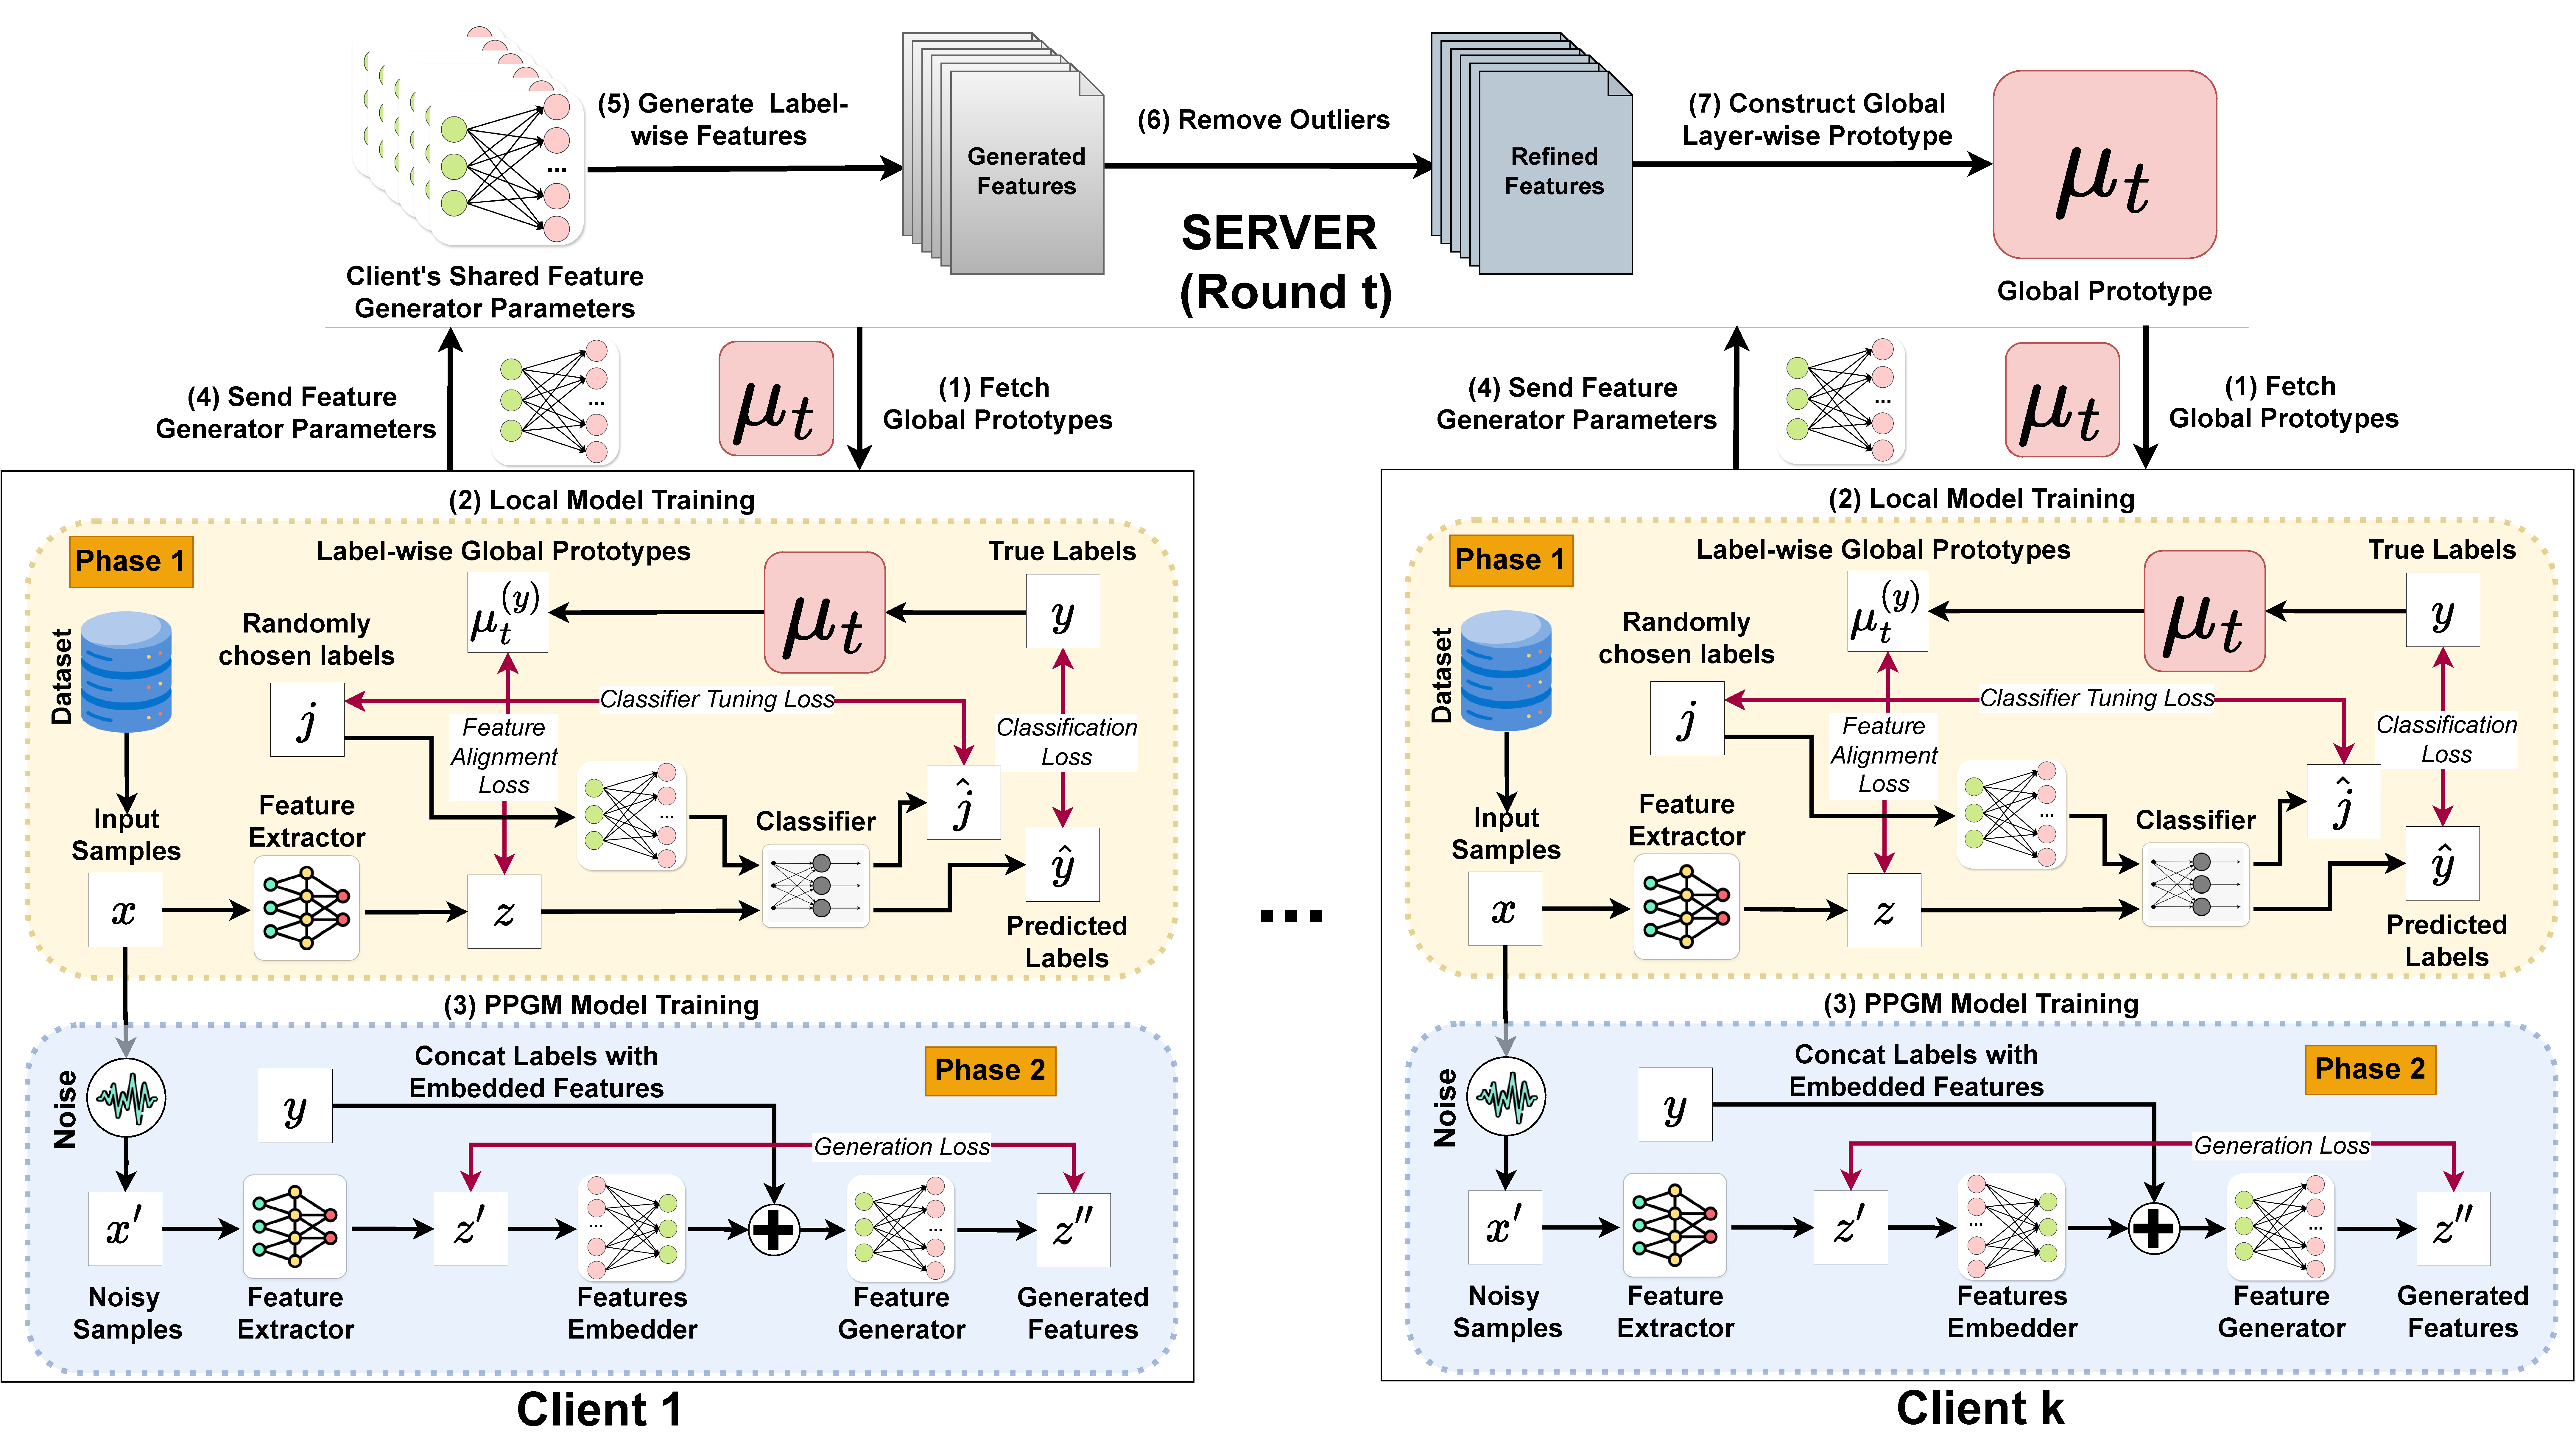
\includegraphics[width=\textwidth]{protogen_corrected-Page-7.pdf}
\end{center}
\caption{An overview of \textsf{ProtoGen} learning framework. The learning process consists of the following steps: (1) clients fetch global prototypes from the server; (2) clients perform local model training with feature alignment and classification losses; (3) clients train the \emph{PPGM} model using noisy local data; (4) clients send feature generator parameters to the server; (5) the server generates label-wise features using received generators; (6) outliers are removed from the generated features; and (7) the server constructs updated global prototypes for the next round.}
\label{fig:framework_overview}
\end{figure*}


\section{\textsf{ProtoGen}: Proposed FL Approach}
\label{sec:methodology}

This section presents our proposed FL framework, \textsf{ProtoGen}, which adapts prototype learning to mitigate data heterogeneity by aligning local hidden features with the global class-wise features prototype. Figure \ref{fig:framework_overview} depicts the overall \textsf{ProtoGen} framework, which introduces the following key components: (1) a novel privacy-preserving feature generation module for each client to capture local hidden feature distribution from the local raw data without compromising privacy, and (2) a global class-wise feature prototype construction mechanism to obtain a generalized global representation via features distillation from client's shared feature generator parameters. In each round $t$, clients fetch $\mu_t$ from the server and train their local models in Phase 1 to minimize the local objective. Following this, in Phase 2, clients train the privacy-preserving generative module using hidden features ($\mathcal{Z'}$) extracted from noisy local data ($\mathcal{X'}$) and shares the associated features generator parameters $\psi$ with the server. Finally, the server constructs global class-wise features prototype $\mu_{t+1}$ for the next round by distilling robust features from the shared $\psi$.


\subsection{Problem Statement}
\bgroup
Consider a federated learning environment with a set of clients $\displaystyle \sK$, where each client $k \in \displaystyle \sK$ has a local dataset $\displaystyle \sD_k = \{(x^i_{k}, y^i_{k})\}_{i=1}^{n_k}$, where $n_k$ is the total number of data samples with client $k$. The data samples $x^i_{k} \in \mathcal{X}_k$ and labels $y^i_{k} \in \mathcal{Y}_k$ are drawn from client-specific distributions $p_k(x, y)$. In the non-IID setting, the distributions $p_k$ can differ significantly across clients. The goal is to learn a generalized local model $\mathcal{F}(\theta_k, \mathcal{X}_k) \rightarrow \mathcal{Y}_k$ parameterized by $\theta_k$ that performs well under heterogeneous data distributions. This model consists of two main components: feature extractor and classifier. The feature extractor, parameterized by $\phi_k$,  transforms raw input data $\mathcal{X}_k$ into a feature space $\mathcal{Z}_k$, formally defined as: $\mathcal{H}(\phi_k, \mathcal{X}_k)\rightarrow \mathcal{Z}_k$. The classifier, parameterized by $\varphi_k$, takes the extracted feature representation $z=\mathcal{H}(\phi_k, x)$ to predict the corresponding class label, formally expressed as $ \hat{y} = \mathcal{C}(\varphi_k, z)$, where $x  \in \mathcal{X}_k, z \in \mathcal{Z}_k$. 
Additionally, clients train a privacy-preserving generative module $\mathcal{G}(\psi_k, \mathcal{Y}_k) \rightarrow \mathcal{Z}_k$, parameterized by $\psi_k$, is introduced to synthesize features that resemble those produced by $\mathcal{H}(\phi_k, x')$, where $x'$ is the noisy data. To enhance privacy, Gaussian noise $\epsilon \sim \mathcal{N}(0, \sigma^2)$ is added to the input, forming a perturbed version $x' = x + \epsilon$. The overall training objective is defined as follows:

\begin{align}
    \min_{\phi_k, \varphi_k, \psi_k} & \mathbb{E}_{(x, y) \sim p_k(x, y)} \left[ \mathcal{L}_{CE}(\mathcal{C}(\varphi_k, \mathcal{H}(\phi_k, x)), y) \right. \\ \nonumber
    & + \lambda_a \| \mathcal{H}(\phi_k, x) - \mu^{(y)} \|^2  \left. + \mathcal{D} (\mathcal{G}(\psi_k, y), \mathcal{H}(\phi_k, x')) \right]
\end{align}

where $\mathcal{D}(\cdot, \cdot)$ is a similarity metric such as Mean Squared Error, $\mu^{(y)}$ is the global class-wise prototype for class label $y$ received from the server, and $\lambda_a$ controls the strength of feature alignment.
 $\mathcal{L}_{CE}: \hat{\mathcal{Y}} \times \mathcal{Y} \rightarrow \mathbb{R}_+$ is the local objective function, e.g. cross-entropy loss for classification task.


\subsection{Client's Local Training}
Each client $k\in\sK$ performs local training in the following two phases:

\noindent\textbf{Phase 1 (Minimizing Local Objective):} In this phase, each client $k\in \sK$ trains its local classification module through a combined objective function $\mathcal{L}_{C}$ that effectively balances three learning objectives: supervised classification, hidden features alignment, and synthetic feature-based classifier tuning. The supervised classification loss $\mathcal{L}_{CE} (\mathcal{C}(\varphi_{k,t}, \mathcal{H}(\phi_{k,t}, x)), y)$ is to ensure accurate predictions on local data, whereas hidden features alignment loss $\| \mathcal{H}(\phi_{k,t}, x) - \mu_t^{(y)} \|^2$ is to ensure that the input's hidden features $\mathcal{H}(\phi_{k,t}, x)$ align with the global class-wise feature prototypes $\mu_t$ received from the server. This alignment helps the client to mitigate the impact of data heterogeneity across clients via distilling global knowledge from class-wise feature prototypes. Additionally, to address label imbalance and mitigate classifier bias, each client randomly samples a class label \(j \in \sC\), where \(\sC\) denotes the global set of unique classes, and subsequently the client synthesizes representative features \(\mathcal{G}(\psi_k^t, j)\), which are then passed to the classifier to compute an auxiliary classifier tuning loss $\mathcal{L}_{CE} (\mathcal{C}(\varphi_{k,t}, \mathcal{G}(\psi_{k,t}, j)), j)$. Utilizing the above three key learning objectives, we define the combined objective function $\mathcal{L}_{C}$ of local training as:
\begin{align}
\label{eq:combined_objective}
\mathcal{L}_{C} &= \mathcal{L}_{CE} (\mathcal{C}(\varphi_{k,t}, \mathcal{H}(\phi_{k,t}, x)), y) + \lambda_{a} \| \mathcal{H}(\phi_{k,t}, x) - \mu_t^{(y)} \|^2 \\ \nonumber
& \quad \quad \quad \quad \quad \quad\quad \quad + \lambda_{c}\mathcal{L}_{CE} (\mathcal{C}(\varphi_{k,t}, \mathcal{G}(\psi_{k,t}, j)), j)
\end{align}
where $\mathcal{L}_{CE}$ represents the cross-entropy loss, $\mathcal{H}(\phi_{k,t}, x)$ is the feature extractor, $\mathcal{C}(\varphi_{k,t}, \cdot)$ is the classifier, and $\lambda{a}$ and $\lambda_{c}$ are hyper-parameters controlling the importance of feature alignment and generated feature classification, respectively.

At each communication round \(t\), the client updates its local model parameters \(\theta_{k,t} = \{\phi_{k,t}, \varphi_{k,t}\}\), where \(\phi_k^t\) and \(\varphi_{k,t}\) represent feature extractor and classifier parameters, respectively. The parameters are optimized by minimizing the combined loss \(\mathcal{L}_C\) via gradient descent with a local learning rate \(\eta_l\), formally defined as:
\begin{align}
\label{eq:local_update}
    \theta_{k,t+1} \leftarrow \theta_{k,t} - \eta_l \nabla_{\theta_{k,t}} \mathcal{L}_C
\end{align}


\begin{algorithm}[t]
\caption{Training Feature Generation Module}
\label{alg:phase2}
\begin{algorithmic}[1]
\State \textbf{Input:} Client dataset $\sD_k$, feature generator $\mathcal{G}_k$, main model's feature extractor $\mathcal{H}_k$, hyper-parameters $\lambda_{gen}$, $\lambda_{kl}$, \emph{PPGM} learning rate $\eta_{gen}$, and number of epochs $E$.
% \State \textbf{Output:} Trained model parameters $\psi_k$
% \State \textbf{Initialize:} \emph{PPGM} model parameters $\varphi$ for classifier $\mathcal{C}$, feature transformation parameters $\phi$, and feature generator $\psi$.
\State \textbf{\emph{PPGM} Model Training:}
\For{\textcolor{cyan}{each local epoch} $e = 1, 2, \dots, E$}
    \For{\textcolor{magenta}{each batch} $(x, y) \in \sD_k$}
    \State \textbf{Add} gaussian noise: $x' \leftarrow x + \mathcal{N}(0, \sigma^2)$
    \State \textbf{Compute} local feature: $z \leftarrow \mathcal{H}(\phi_k, x')$
    \State \textbf{Compute} generation Loss: 
    % $\mathcal{L}_{GEN} \leftarrow \lambda_{gen}\mathcal{D}(\mathcal{G}(\psi, y), z) + \lambda_{kl}\text{KL}(q_{\psi}(z|y) | p(z))$
    $\mathcal{L}_{GEN} \leftarrow \lambda_{gen}\mathcal{D}(\mathcal{J}(\varrho_k, \mathcal{E}(\rho_k,z|y)|y), z) + \lambda_{kl}\text{KL}(\mathcal{E}_{\rho_k}(e|z,y) | p(e))$
    \State \textbf{Update} generative model parameters: $\psi_{k}^{e+1} \leftarrow \psi_{k}^{e} - \eta_{gen} \nabla_{\psi_{k}^{e}} \mathcal{L}_{GEN}$
    \EndFor
\EndFor
\State \textbf{Return:} Trained model parameters $\psi_k$
\end{algorithmic}
\end{algorithm}

\noindent\textbf{Phase 2: (Training of Privacy-Preserving Generative Module)}
To facilitate the sharing of client's knowledge while preserving privacy, each client trains a feature generator $\mathcal{G}(\psi, y)$. Gaussian noise $\epsilon$ is first added to input $x$ to form $x'$, and the feature extractor then maps $x'$ to features $z' = \mathcal{H}(\phi, x')$. 
The generator is trained to approximate this mapping:
\begin{equation}
    \min_{\psi} \mathbb{E}_{(x, y) \sim p_k(x, y)} \left[ \mathcal{D} (\mathcal{G}(\psi, y), \mathcal{H}(\phi, x')) \right]
\end{equation}

where $\mathcal{D}(\cdot, \cdot)$ is a similarity metric such as Mean Squared Error. Once training is complete, only the required feature generation parameters of $\mathcal{G}$ are shared with the server, preserving privacy (e.g., only decoder parameters are shared when using VAE as a generative module). This is worth noting that, even though this paper considers a Conditional Variational Autoencoder (CVAE) like architecture, the proposed framework is flexible enough to accommodate other generative models such as GANs, diffusion, etc., \cite{10.1145/3422622, ho2020denoisingdiffusionprobabilisticmodels}.

% \begin{figure}[t]
%     \centering
%     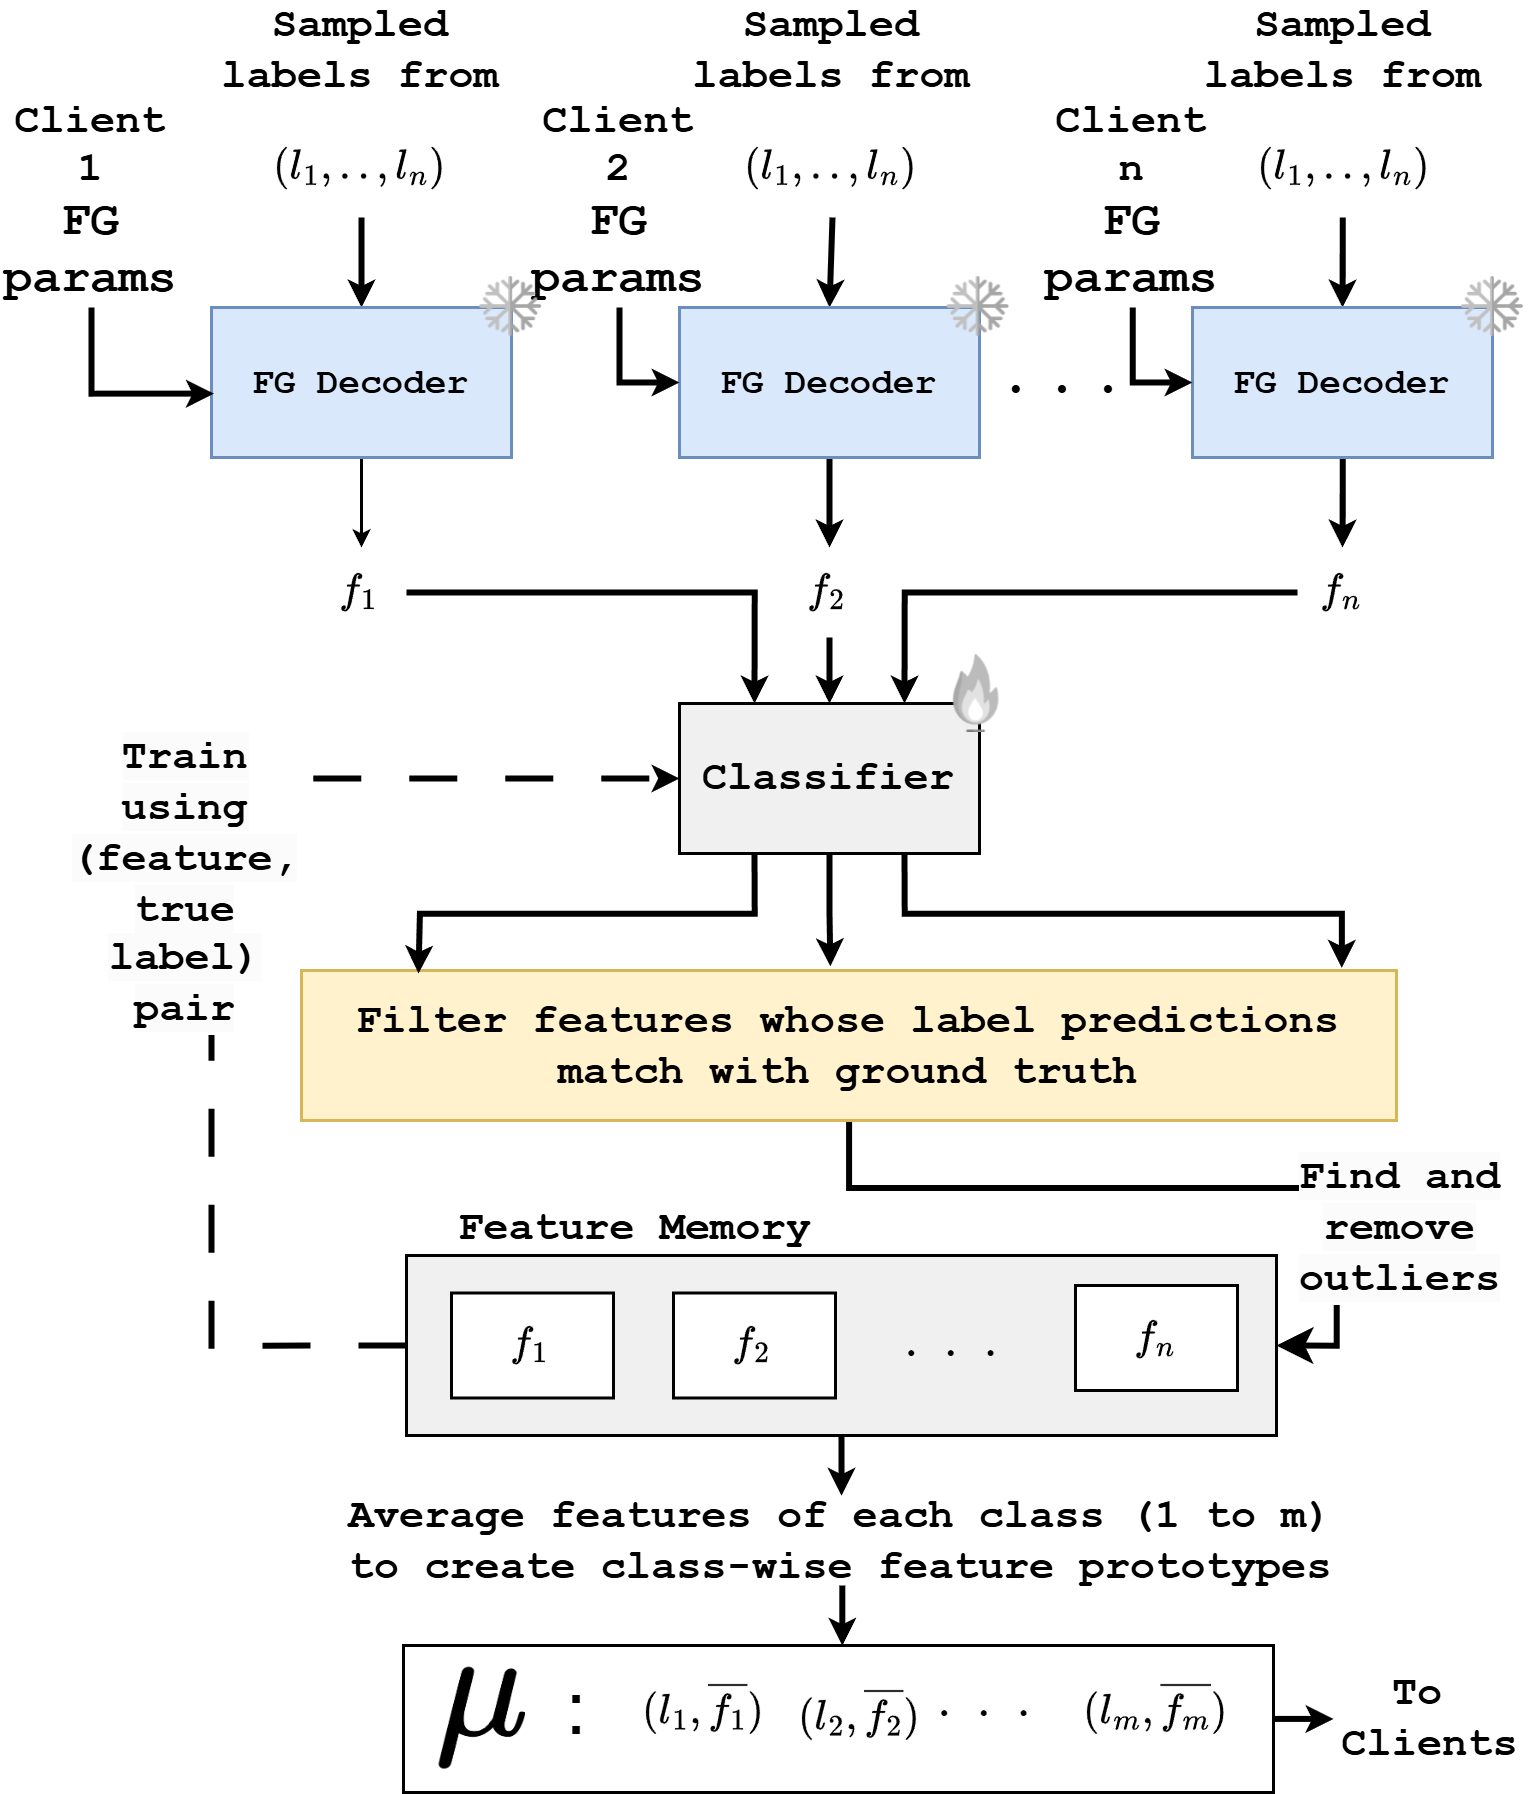
\includegraphics[width=\columnwidth]{images/fedflair-Server.png}  % Use your image file
%     \caption{An Overview of Server Side Prototype Construction}
%     \label{fig:server}
% \end{figure}

\noindent\paragraph*{CVAE for Feature Generation}
To facilitate knowledge sharing while preserving privacy, each client trains a conditional variational autoencoder (CVAE) as the feature generator $\mathcal{G}(\psi, y)$. The CVAE learns to generate class-conditional features that closely resemble the distribution of real features extracted by the feature extractor $\mathcal{H}$. The CVAE consists of an encoder $\mathcal{E}(\rho, z|y)$ and a decoder $\mathcal{J}(\varrho, e|y)$, where $\rho$ and $\varrho$ are the encoder and decoder parameters, respectively.
During training, Gaussian noise $\epsilon \sim \mathcal{N}(0, \sigma^2)$ is first added to input $x$ to form $x'$, and the feature extractor then maps $x'$ to features $z'=\mathcal{H}(\phi, x')$. The encoder maps these features and class labels to a latent distribution parameterized by mean $\nu$ and variance $\sigma^2$, from which a latent code $e$ is sampled using the reparameterization trick. The decoder then reconstructs the features conditioned on the latent code and class label.
The training objective combines reconstruction loss and KL divergence:
\begin{align}
\min_{\rho, \varrho} \mathbb{E}{(x, y) \sim p_k(x, y)} & \left[ \lambda_{gen}\mathcal{D}(\mathcal{J}(\varrho, \mathcal{E}(\rho,z|y)|y), z) \right. \\ \nonumber
&+ \left. \lambda_{kl}\text{KL}(\mathcal{E}_{\rho}(e|z,y) | p(e))  \right]
\end{align}
where $\mathcal{D}(\cdot, \cdot)$ is the mean squared error loss between the generated features and the features extracted from noise-perturbed inputs, $\text{KL}(\cdot | \cdot)$ represents the Kullback-Leibler divergence that encourages the learned latent distribution $\mathcal{E}_{\rho}(e|z,y)$ to be close to a prior distribution $p(e)$ (typically a standard normal distribution), thereby promoting the generation of diverse features. The hyper-parameters $\lambda_{gen}$ and $\lambda_{kl}$ control the importance of each loss component.

Upon completion of generative module training, clients share only the decoder parameters $\varrho$ with the server, preserving data privacy while enabling effective knowledge transfer through the learned feature distributions. This approach significantly reduces communication overhead compared to sharing full model parameters, as the decoder is typically much smaller than the complete model.

\subsection{Server's Knowledge Distillation and Prototype Construction}
At the server, the received feature generator parameters from all clients are used to synthesize class-wise feature representations. These synthetic features are then processed through an outlier removal mechanism to eliminate noisy or unrepresentative samples, resulting in a more reliable set of robust features. Using these robust features, the server constructs a global class-wise features prototype for each class $c\in \sC$ by averaging features synthesized across contributing clients:
\begin{equation}
\label{eq:global_proto}
\mu = \left\{\mu^{(c)} | \mu^{(c)} = \frac{1}{|\sK|} \sum_{k \in \sK}  \frac{1}{|y^{(c)}|}\sum_{y_j\in y^{(c)}}\mathcal{J}(\varrho_k, y_j) \right\}_{c\in \sC}    
\end{equation}
where $y^{(c)}$ denotes the list of labels $c$. 
The resulting global prototype set \(\mu\) serves as a distilled representation of feature-level knowledge aggregated from the federation. It helps to mitigate the effects of data heterogeneity and enables consistent semantic alignment across clients.

In subsequent training rounds, the server distributes the global prototypes \(\mu\) to the selected clients. Each client then uses these prototypes to guide the training of its local feature extractor. This is achieved by minimizing the discrepancy between its locally extracted features and the corresponding global class prototypes through the following alignment loss:
\begin{equation}
    \mathcal{L}_{algn} = \mathbb{E}_{(x, y) \sim p_k(x, y)} \left[ \| \mathcal{H}(\phi, x) - \mu^{(y)} \|^2 \right]
\end{equation}
This iterative process ensures that local models learn a unified feature space while maintaining privacy and minimizing communication overhead. As a result, \textsf{ProtoGen} effectively addresses data heterogeneity and enhances generalization in federated learning environments.

\begin{algorithm}[t]
\caption{\textsf{ProtoGen}: Federated Privacy-Preserving Prototype Learning via Feature Generation}
\label{algo:ProtoGen}
\begin{algorithmic}[1]
    \State \textbf{Input:} Number of clients $\sK$, number of communication rounds $T$, local datasets $\{\sD_k|k \in \sK\}$, local model learning rate $\eta_l$    
    % \State \textbf{\textcolor{myorange}{Output:}} Generalized and robust local model parameters ( $\Theta_k|k\in\sK$ )
    \State \textbf{Federated Training:}
    \For{\textcolor{mygreen}{each communication round} $t = 1, \dots, T$}
        \State \textbf{Select} a set of clients $\sS_t$ for local training.
        \State \textbf{\textcolor{myred}{Local Training:}}
        \For{\textcolor{mygreen}{each client} $k \in \sS_t$ \textbf{in parallel}}
            \For{\textcolor{cyan}{epocs} $e = 1, \dots, E$}
                \State \textbf{Sample} a batch of local dataset $\{ x , y\} \in \sD_k$
                \State \textbf{Compute} local features: $z \leftarrow \mathcal{H}(\phi, x)$
                \State \textbf{Choose} random labels: $j \in \sC$
                \State \textbf{Generate} synthetic features $z_{gen} \leftarrow \mathcal{G}(\psi_k, j) $
                \State \textbf{Update} local model parameters following Equation~\ref{eq:local_update}.
            \EndFor
            \State \textbf{Update} local generation module parameters ($\psi_{k,t}$) following Algorithm~\ref{alg:phase2}.
            \State \textbf{Send} feature generator parameters ($\varrho_{k,t+1}$) to the server.
        \EndFor
        \State \textbf{\textcolor{myred}{Aggregation:}}
        \State \textbf{Compute} global class-wise prototype following Equation \ref{eq:global_proto}.
    \EndFor

    % \State \Return \textcolor{myblue}{Global model $f_{\theta_T}$}
\end{algorithmic}
\end{algorithm}

Algorithm \ref{algo:ProtoGen} outlines the overall \textsf{ProtoGen} training process across multiple clients. The algorithm begins with initialization of local models and feature generators across all clients (line 1). For each communication round, the server randomly selects a subset of clients to participate for local training (line 4), and each selected client update their local model over multiple epochs (lines 6-13). During each epoch, clients sample batches from their local datasets, compute local features using the feature extractor, choose random class labels to mitigate classifier drift, generate synthetic features for the chosen class labels using the feature generator, and update local model parameters following Equation \ref{eq:local_update}. After completing local model training, each client updates its feature generation module parameters following Algorithm \ref{alg:phase2} and sends only the generative portion of its updated parameters to the server (lines 14-15). The server then aggregates the received generators to construct updated global class-wise prototypes following Equation \ref{eq:global_proto} (line 18). This process repeats until convergence or a maximum number of rounds is reached.

This design significantly improves communication efficiency by sharing only the feature generator parameters $\varrho$ instead of the entire generative model parameters, which significantly reduces bandwidth requirements compared to traditional federated learning methods. Further, sharing of abstract generative capabilities rather than raw features from sensitive client data enhances privacy guarantees in the system. The bidirectional exchange of feature generators and class-wise prototypes fosters robust knowledge transfer across heterogeneous client distributions, effectively addressing key challenges in FL, such as non-IID data, class imbalance, and missing class scenarios. As a result, clients can leverage collective knowledge while retaining data privacy, promoting a more equitable and generalizable FL environment.

\subsection{\textsf{ProtoGen}$^+$}

To further reduce the communication cost of our approach, we propose an enhanced variant called \textsf{ProtoGen}$^+$. Instead of transmitting privacy-preserved feature generator parameters to the server, each client independently constructs class-wise feature prototypes using the locally trained \emph{PPGM} module.
Specifically, client $k$ constructs local class-wise prototypes $\mu_k$ as:
\begin{equation}
    \label{eq:local_proto}
    \mu_k = \left\{\mu_k^{(c)} \,\big|\, \mu_k^{(c)} = \frac{1}{n_k^{(c)}} \sum_{ y_{k,j}^{(c)}\in \mathcal{D}_k^{(c)}} \mathcal{J}(\varrho_k,  y_{k,j}^{(c)}) \right\}_{c \in \mathcal{C}}
\end{equation}

where $\mathcal{D}_k^{(c)} = \{(x_{k,j}^{(c)}, y_{k,j}^{(c)}) \mid j = 1, 2, \ldots, n_k^{(c)}\}$ represents the subset of data samples belonging to class $c$ at client $k$. Here, $x_{k,j}^{(c)}$ denotes the $j$-th feature vector of class $c$ at client $k$, and $ y_{k,j}^{(c)}$ its corresponding class label. $n_k^{(c)} = |\mathcal{D}_k^{(c)}|$ represents the number of samples of class $i$ at client $k$. The function $\mathcal{J}(\varrho_k, y_{k,j}^{(c)})$ denotes the feature representation generated by the client's \emph{PPGM} module's features generator parameters $\varrho_k$ for label $ y_{k,j}^{(c)}$.
Once the local prototypes $\mu_k$ are constructed, they are transmitted to the server. The server then aggregates the received local prototypes across all participating clients $\mathcal{K}$ to compute global class-wise prototypes $\mu$ as follows:

\begin{equation}
\label{eq:global_proto_plus}
\mu = \left\{\mu^{(c)} \,\big|\, \mu^{(c)} = \frac{1}{|\mathcal{K}|} \sum_{k \in \mathcal{K}} \mu_k^{(c)} \right\}_{c \in \mathcal{C}}    
\end{equation}

where, $\mu_k^{(c)}$ denotes the prototype for class $c$ from client $k$. The resulting global class-wise features prototypes $\mu$ are then shared with clients for the subsequent round of federated learning.

This prototype-based communication scheme not only reduces the communication cost per round but also significantly lowers the server-side computation overhead. Unlike the original \textsf{ProtoGen}, where the server had to regenerate class-wise features from each client's generator parameters, \textsf{ProtoGen}$^+$ simplifies the process by directly using aggregated prototypes. However, this comes at the cost of  some compromise in privacy as during local-prototype sharing clients will reveal which class samples are present in their corresponding local trainset.


\section{Theoretical Analysis of \textsf{ProtoGen}}\label{sec-th}

This section presents the following theorems, which collectively demonstrate the theoretical foundations of \textsf{ProtoGen}.

\subsection{Preliminaries and Notation}

Let $\sK$ be the set of all clients, with $|\sK| = K$. For each client $k \in \sK$, let $\sD_k$ be its local dataset, with $n_k = |\sD_k|$ and $n = \sum_{k=1}^K n_k$. Let $\theta_{k,t} \in \mathbb{R}^d$ denote the local model parameters of client $k$ at round $t$. Let $\rho_{k,t} \in \mathbb{R}^p$ and $\varrho_{k,t} \in \mathbb{R}^q$ denote the \emph{PPGM} encoder and decoder parameters of client $k$ at round $t$, respectively. $\psi_k \leftarrow\{\rho_k,\varrho_k\}$ represents the general \emph{PPGM} model parameters of client $k$. 

We define the following:
\begin{itemize}
    \item $\mathcal{L}_C(\theta; x, y)$: loss function for client models
    % \item $\mathcal{L}_{\emph{GEN}}(\rho, \varrho; x, y)$: loss function for \textsf{PPGM}
    \item $\mathcal{L}_{\emph{GEN}}(\psi; x, y)$: loss function for \emph{PPGM}
    \item $\mathcal{T}(\theta_k) = \mathbb{E}_{(x,y)\sim\sD_k}[\mathcal{L}_C(\theta_k; x, y)]$: expected combined local objective loss for client $k$
    % \item $\mathcal{V}(\rho_k, \varrho_k) = \frac{1}{K}\sum_{k=1}^K \mathbb{E}_{(x,y)\sim\sD_k}[\mathcal{L}_{\emph{PPGM}}(\rho, \varrho; x, y)]$: expected feature generation loss for client $k$.
    \item $\mathcal{V}(\psi_k) = \frac{1}{K}\sum_{k=1}^K \mathbb{E}_{(x,y)\sim\sD_k}[\mathcal{L}_{\emph{GEN}}(\psi_k; x, y)]$: expected feature generation loss for client $k$.
\end{itemize}

\subsection{Assumptions}

We make the following assumptions:

\begin{assumption}[Smoothness]
\label{asm:1}
$\mathcal{T}(\theta_k)$ is $L$-smooth for all $k$: $\forall \theta_k, \theta'_k \in \mathbb{R}^d$,
\begin{equation}
    \|\nabla \mathcal{T}(\theta_k) - \nabla \mathcal{T}(\theta'_k)\| \leq L_1\|\theta_k - \theta'_k\|
\end{equation}
where $L_1 > 0$ is the Lipschitz constant for the local model.
\end{assumption}


\begin{assumption}[Strong Convexity]
\label{asm:2}
$\mathcal{T}(\theta_k)$ is $\mu$-strongly convex for all $k$: $\forall \theta_k, \theta'_k \in \mathbb{R}^d$,
\begin{equation}
    \mathcal{T}(\theta'_k) \geq \mathcal{T}(\theta_k) + \langle\nabla \mathcal{T}(\theta_k), \theta'_k - \theta_k\rangle + \frac{\mu}{2}\|\theta'_k - \theta_k\|^2
\end{equation}
\end{assumption}

\begin{assumption}[Bounded Variance]
\label{asm:3}
The variance of stochastic gradients is bounded for both client models and \emph{PPGM}, $\forall k \in \sK, \forall \theta_k \in \mathbb{R}^d$:
\begin{equation}
    \mathbb{E}_{(x,y)\sim\sD_k}[\|\nabla\mathcal{L}_C(\theta_k; x, y) - \nabla \mathcal{T}(\theta_k)\|^2] \leq \sigma_1^2
\end{equation}
% Similarly, $, \quad \forall k \in \sK, \forall \phi_k, \psi_k$
\begin{equation}
    \mathbb{E}_{(x,y)\sim \sD_k}[\|\nabla\mathcal{L}_{\emph{GEN}}(\psi_k; x, y) - \nabla \mathcal{V}(\psi_k)\|^2] \leq \sigma_2^2
\end{equation}
\end{assumption}

\begin{assumption}[\emph{PPGM} Lipschitz Continuity]
\label{asm:4}
The \emph{PPGM} model is Lipschitz continuous with respect to its parameters:
\begin{equation}
% \begin{split}    
    \|\nabla \mathcal{V}(\psi_k) - \nabla \mathcal{V}(\psi_k') \| \leq L_2(\|\psi_k - \psi_k'\|)
% \end{split}
\end{equation}
where $L_2 > 0$ is the Lipschitz constant for the \emph{PPGM} model.
\end{assumption}

\begin{assumption}[Gradient Dissimilarity]
\label{asm:5}
For each client \( k \in \sK \), assume that the loss function \( \mathcal{T}(\theta_k) \) is differentiable and bounded below, with \( \theta_{k,t} \) denoting the model parameters at round \( t \), and \( \theta_k^* \) being a minimizer of \( \mathcal{T}(\theta_k) \). Then, there exist constants \( G \geq 0 \) and \( \beta \geq 0 \) such that:
\begin{equation}
\frac{1}{K}\sum_{k=1}^K \|\nabla \mathcal{T}(\theta_{k,0}) - \nabla \mathcal{T}(\theta_k^*)\|^2 
\leq G^2 + 2\beta \left( \mathcal{T}(\theta_{k,0}) - \mathcal{T}(\theta_k^*) \right)
\end{equation}
where \( G^2 \) is a non-negative constant that upper bounds the inherent variance in the client gradients (even near local optima), \( \beta \) is a non-negative constant that quantifies how gradient differences grow with suboptimality (i.e., how far \( \theta_{k,t} \) is from \( \theta_k^* \) in terms of objective value).

\end{assumption}


\subsection{Convergence Analysis}
\begin{lemma}[One-step Progress for Client Models]
\label{lemma:1}
For client $k \in \sK$, gradient computed with learning rate $\eta_l$ over $E$ local epochs at round $t \geq 0$, its one-step convergence bound follows:
\begin{equation}
\begin{split}
    &\mathbb{E}[\|\theta_{k,t+1} - \theta_k^*\|^2] \leq (1-\mu\eta_l)\mathbb{E}[\|\theta_{k,t}  - \theta_k^*\|^2]\\
    & \qquad - 2\eta_l\mathbb{E}[\mathcal{T}(\theta_{k,t}) - \mathcal{T}(\theta_k^*)]\\ 
    & \qquad \quad + \eta_l^2\left(\sigma_1^2 + 6L\gamma_1 E\eta_l + 8(E-1)^2\gamma_1^2\right)
\end{split}
\end{equation}
where $\gamma_1 = \max\{\frac{8L_1}{\mu}, E\}$
\end{lemma}

\begin{proof}
Detailed proof is reported in the supplementary document attached with this manuscript, due to space constraints.

% Let $g_{k,t}$ be the average stochastic gradient computed by client $k$ at round $t$ over $E$ local epochs. The update rule for client $k$'s model parameters is $\theta_{k,t+1} = \theta_{k,t} - \eta_l g_{k,t}$. We begin by expanding $\|\theta_{k,t+1} - \theta_k^*\|^2$:

% \begin{align*}
% \|\theta_{k,t+1} - \theta_k^*\|^2 &= \|\theta_{k,t} - \eta_l g_{k,t} - \theta_k^*\|^2 \\
% &= \|\theta_{k,t} - \theta_k^*\|^2 - 2\eta_l \langle g_{k,t}, \theta_{k,t} - \theta_k^* \rangle\\ 
% & \qquad+ \eta_l^2 \|g_{k,t}\|^2
% \end{align*}

% Taking the expectation of both sides:

% \begin{align*}
% \mathbb{E}[\|\theta_{k,t+1} - \theta_k^*\|^2] &= \mathbb{E}[\|\theta_{k,t} - \theta_k^*\|^2] - 2\eta_l \mathbb{E}[\langle g_{k,t}, \theta_{k,t} - \theta_k^* \rangle]\\ 
% & \qquad \qquad + \eta_l^2 \mathbb{E}[\|g_{k,t}\|^2]
% \end{align*}

% Using the strong convexity and smoothness of $T(\theta_k)$, we can bound the inner product term:

% \begin{align*}
% \langle g_{k,t}, \theta_{k,t} - \theta_k^* \rangle &\geq \mathcal{T}(\theta_{k,t}) - \mathcal{T}(\theta_k^*) + \frac{\mu}{2}\|\theta_{k,t} - \theta_k^*\|^2\\ 
% &\qquad - \langle g_{k,t} - \nabla \mathcal{T}(\theta_{k,t}), \theta_{k,t} - \theta_k^* \rangle
% \end{align*}

% For the gradient norm, we use the smoothness property and the definition of $\gamma_1$:

% \begin{equation}
% \mathbb{E}[\|g_{k,t}\|^2] \leq 4L_1(\mathcal{T}(\theta_{k,t}) - \mathcal{T}(\theta_k^*)) + 2\sigma_1^2 + 2\gamma_1^2
% \end{equation}

% Combining these bounds and applying Cauchy-Schwarz inequality to the error term, we get:
% \begin{align*}
% \mathbb{E}[\|\theta_{k,t+1} - \theta_k^*\|^2] &\leq (1 - 2\mu\eta_l)\mathbb{E}[\|\theta_{k,t} - \theta_k^*\|^2]\\ 
% &- 2\eta_l(1 - \eta_l L_1)\mathbb{E}[\mathcal{T}(\theta_{k,t}) - \mathcal{T}(\theta_k^*)] \\
% &\quad + \eta_l^2(2\sigma_1^2 + 2\gamma_1^2) + \eta_l\sigma_1^2
% \end{align*}

% To account for $E$ local epochs, we model this as $E$ consecutive updates with learning rate $\eta_l$. Applying the above inequality $E$ times and using the convexity of $\mathcal{T}(\theta_k)$, we get the following:

% \begin{align*}
% % \centering
% &\mathbb{E}[\|\theta_{k,t}^E - \theta_k^*\|^2] \leq (1 - 2\mu\eta_l)^E\mathbb{E}[\|\theta_{k,t} - \theta_k^*\|^2]\\ 
% & \qquad \qquad - 2E\eta_l(1 - \eta_l L_1)\mathbb{E}[\mathcal{T}(\theta_{k,t}) - \mathcal{T}(\theta_k^*)] \\
% &\qquad \qquad \quad + E\eta_l^2(2\sigma_1^2 + 2\gamma_1^2) + E\eta_l\sigma_1^2\\ 
% &\qquad \qquad \qquad + 4L_1\eta_l^2E(E-1)\gamma_1^2
% \end{align*}


% Finally, using the fact that $\eta_l \leq 1/(4L_1)$ (which follows from our choice of $\eta_l$) and combining like terms, we obtain the stated bound:

% \begin{equation}
% \begin{split}
% \mathbb{E}[\|\theta_{k,t+1} - \theta_k^*\|^2] \leq& (1-\mu\eta_l)\mathbb{E}[\|\theta_{k,t} - \theta_k^*\|^2]\\ 
% &- 2\eta_l\mathbb{E}[\mathcal{T}(\theta_{k,t}) - \mathcal{T}(\theta_k^*)] \\
% &+ \eta_l^2(\sigma_1^2 + 6L\gamma E\eta_l + 8(E-1)^2\gamma_1^2)
% \end{split}
% \end{equation}

\end{proof}

\begin{lemma}[One-step Progress for \emph{PPGM}]
\label{lemma:2}
For any round $t \geq 0$, the convergence bound for \emph{PPGM} follows:
\begin{equation}
\begin{split}
    \mathbb{E}[\|\psi_{k,t+1} - \psi_k^*\|^2]
    &\leq \mathbb{E}[\|\psi_{k,t} - \psi_k^*\|^2]\\
    &\quad - 2\eta_g \mathbb{E}[\mathcal{V}(\psi_{k,t}) - \mathcal{V}(\psi_k^*)] \\
    &\quad - \frac{\eta_g}{L_2} \sigma_2^2 + \eta_g^2 \sigma_2^2
\end{split}
\end{equation}
\end{lemma}


\begin{proof}
Detailed proof is reported in the supplementary document attached with this manuscript, due to space constraints.

% Let $g'_t = \nabla \mathcal{V}(\psi_{k,t})$ be the gradient of the \emph{PPGM} loss function at round $t$. The update rule for $\psi_k$ with learning rate $\eta_g$ defined as:
% \begin{equation}
% \psi_{k,t+1} = \psi_{k,t} - \eta_g g'_t
% \end{equation}
% % For simplicity, we denote $\mathbb{E}[\|\rho_{k,t+1} - \rho_k^*\|^2 + \|\varrho_{k,t+1} - \varrho_k^*\|^2]$ as $\|(\rho_{k,t+1}, \varrho_{k,t+1}) - (\rho_k^*, \varrho_k^*)\|^2$.\\
% We begin by expanding $\|\psi_{k,t+1} - \psi_k^*\|^2$:

% \begin{align*}
% &\|\psi_{k,t+1} - \psi_k^*\|^2 = \|\psi_{k,t} - \eta_g g'_t - \psi_k^*\|^2 \\
% &= \|\psi_{k,t} - \psi_k^*\|^2 - 2\eta_g \langle g'_t, \psi_{k,t} - \psi_k^* \rangle + \eta_g^2 \|g'_t\|^2
% \end{align*}

% Taking the expectation of both sides:

% \begin{equation}
% \label{eq:21}
% \begin{split}
% \mathbb{E}[\|\psi_{k,t+1} - \psi_k^*\|^2] &= \mathbb{E}[\|\psi_{k,t} - \psi_k^*\|^2] \\
% &\qquad- 2\eta_g \mathbb{E}[\langle g'_t, \psi_{k,t} - \psi_k^* \rangle]\\ 
% &\qquad \quad+ \eta_g^2 \mathbb{E}[\|g'_t\|^2]
% \end{split}
% \end{equation}

% By the $L$-smoothness of $Y(\rho_k,\varrho_k)$ with Lipschitz constant $L_2 > 0$, we have:

% \begin{equation}
% \begin{split}
% &\mathcal{V}(\psi_k^*) \geq \mathcal{V}(\psi_{k,t}) + \langle g'_t, \psi_k^* - \psi_{k,t} \rangle + \frac{1}{2L_2}\|g'_t\|^2    
% \end{split}
% \end{equation}

% Rearranging this inequality:

% \begin{equation}
% \label{eq:23}
% \begin{split}
% &\langle g'_t, \psi_k^* - \psi_{k,t} \rangle \geq \mathcal{V}(\psi_{k,t})- \mathcal{V}(\psi_k^*) + \frac{1}{2L_2}\|g'_t\|^2
% \end{split}
% \end{equation}

% Substituting Equation~\ref{eq:23} into Equation~\ref{eq:21}, we have:

% \begin{align*}
% &\mathbb{E}[\|\psi_{k,t+1} - \psi_k^*\|^2] \leq \mathbb{E}[\|\psi_{k,t} - \psi_k^*\|^2]\\
% &\qquad\quad- 2\eta_g \mathbb{E}[\mathcal{V}(\psi_{k,t})- \mathcal{V}(\psi_k^*)]\\ 
% &\qquad \qquad- \frac{\eta_g }{L_2}\mathbb{E}[\|g'_t\|^2]+ \eta_g^2 \mathbb{E}[\|g'_t\|^2]
% \end{align*}

% Now, using the assumption of bounded variance of stochastic gradients, $\mathbb{E}[\|g_t\|^2] \leq \sigma_2^2$, we get:

% \begin{align*}
% &\mathbb{E}[\|\psi_{k,t+1} - \psi_k^*\|^2] \leq \mathbb{E}[\|\psi_{k,t} - \psi_k^*\|^2]\\
% &\qquad\quad- 2\eta_g \mathbb{E}[\mathcal{V}(\psi_{k,t})- \mathcal{V}(\psi_k^*)]\\ 
% &\qquad\qquad - \frac{\eta_g}{L_2} \sigma_2^2 + \eta_g^2 \sigma_2^2
% \end{align*}

\end{proof}

\begin{theorem}[Convergence of \textsf{ProtoGen} in Convex Settings]
\label{theo:1}
Let Assumptions 1-4 hold. Let the learning rates be set as $\eta_l = \frac{2}{\mu(t+\gamma_1)}$ for client models and $\eta_g = \frac{2}{L_2(t+\gamma_2)}$ for the \emph{PPGM}, where $\gamma_1 = \max\{\frac{8L_1}{\mu}, E\}$, $\gamma_2 = \max\{\frac{8L_2}{\mu}, E\}$, and $E$ is the number of local epochs. Then, for $T \geq 1$ number of global rounds of training, the output of \textsf{ProtoGen} satisfies, following convergence bound:
\begin{equation}
\begin{split}
    &\mathbb{E}[\mathcal{T}(\bar{\theta}_{k,T})] - \mathcal{T}(\theta_k^*)\\ 
    &\qquad \leq \frac{4L_1\gamma_1}{\mu T}\left(1 + \log\left(\frac{T}{\gamma_1} + 1\right)\right)
\end{split}
\end{equation}
\begin{equation}
\begin{split}
    &\mathbb{E}[\mathcal{V}(\bar{\psi}_{k,T})] - \mathcal{V}(\psi_k^*)\\ 
    & \qquad \leq \frac{4L_2\gamma_2}{T}\left(1 + \log\left(\frac{T}{\gamma_2} + 1\right)\right)
\end{split}
\end{equation}
where $\bar{\theta}_{k,T} = \frac{1}{T}\sum_{t=1}^T \theta_{k,t}$, $\bar{\psi}_T = \frac{1}{T}\sum_{t=1}^T \psi_t$, and $\theta_k^*, \psi^*$ are the respective optimal parameters.
\end{theorem}


\begin{proof}[Theorem~\ref{theo:1} (Client Model Bound)]
Detailed proof is reported in the supplementary document attached with this manuscript, due to space constraints.

% We first derive the convergence bound for the local model of any client $k$. By Lemma~\ref{lemma:1}, summing over $T$ rounds gives:
% \begin{equation}
% \begin{split}
%     \sum_{t=0}^{T-1} 2\eta_{l,t} \mathbb{E}[\mathcal{T}(\theta_{k,t}) - \mathcal{T}(\theta_k^*)]
%     \leq \|\theta_{k,0} - \theta_k^*\|^2 + \sum_{t=0}^{T-1} \eta_{l,t}^2 C,
% \end{split}
% \end{equation}
% where $C = \sigma_1^2 + 6L_1\gamma_1 E\eta_{l,t} + 8(E-1)^2\gamma_1^2$ and the learning rate is $\eta_{l,t} = \frac{2}{\mu(t + \gamma_1)}$.

% Let $\Delta_t := \mathbb{E}[\mathcal{T}(\theta_{k,t}) - \mathcal{T}(\theta_k^*)]$. Then the inequality becomes:
% \begin{equation}
% \sum_{t=0}^{T-1} \frac{4}{\mu(t + \gamma_1)} \Delta_t \leq D + \sum_{t=0}^{T-1} \frac{4}{\mu^2(t + \gamma_1)^2} C,
% \end{equation}
% where $D = \|\theta_{k,0} - \theta_k^*\|^2$.

% Next, apply Jensen’s inequality and convexity of $\mathcal{T}(\cdot)$:
% \begin{equation}
% \mathbb{E}[\mathcal{T}(\bar{\theta}_{k,T}) - \mathcal{T}(\theta_k^*)] \leq \frac{1}{T} \sum_{t=0}^{T-1} \Delta_t.
% \end{equation}

% We now bound the harmonic and squared harmonic series using integral approximation:
% \begin{align}
%     \sum_{t=0}^{T-1} \frac{1}{t + \gamma_1} &\leq \log\left(\frac{T}{\gamma_1} + 1\right), \\
%     \sum_{t=0}^{T-1} \frac{1}{(t + \gamma_1)^2} &\leq \frac{1}{\gamma_1}.
% \end{align}

% Thus,
% \begin{equation}
% \sum_{t=0}^{T-1} \Delta_t \leq \frac{\mu D}{4} \log\left(\frac{T}{\gamma_1} + 1\right) + \frac{C}{\mu\gamma_1}.
% \end{equation}

% Dividing by $T$, we get:
% \begin{equation}
% \mathbb{E}[\mathcal{T}(\bar{\theta}_{k,T}) - \mathcal{T}(\theta_k^*)]
% \leq \frac{\mu D}{4T} \log\left(\frac{T}{\gamma_1} + 1\right) + \frac{C}{\mu \gamma_1 T}.
% \end{equation}

% By absorbing constants into a single constant (e.g., involving $L_1$), we obtain:
% \begin{equation}
% \mathbb{E}[\mathcal{T}(\bar{\theta}_{k,T})] - \mathcal{T}(\theta_k^*)
% \leq \frac{4L_1\gamma_1}{\mu T} \left(1 + \log\left(\frac{T}{\gamma_1} + 1\right)\right),
% \end{equation}
% which proves the desired bound for client models.
% \end{proof}

% \begin{proof}[Theorem~\ref{theo:1} (\emph{PPGM} Bound)]
% To derive the convergence for the \emph{PPGM} model, we start by summing the result of Lemma~\ref{lemma:2} over all $T$ rounds:

% \begin{equation}
% \label{eq:ppgm-1}
%     \sum_{t=0}^{T-1} 2\eta_g \mathbb{E}[\mathcal{V}(\psi_{k,t}) - \mathcal{V}(\psi_k^*)] 
%     \leq \mathbb{E}[\|\psi_{k,0} - \psi_k^*\|^2] + T\eta_g^2 \sigma_2^2.
% \end{equation}

% Using Jensen's inequality and convexity of $\mathcal{V}(\cdot)$:
% \begin{equation}
% \label{eq:ppgm-2}
%     \mathbb{E}[\mathcal{V}(\bar{\psi}_{k,T}) - \mathcal{V}(\psi_k^*)] 
%     \leq \frac{1}{T} \sum_{t=0}^{T-1} \mathbb{E}[\mathcal{V}(\psi_{k,t}) - \mathcal{V}(\psi_k^*)].
% \end{equation}

% Multiply both sides of Equation~\eqref{eq:ppgm-2} by $2T\eta_g$:
% \begin{equation}
%     2T\eta_g \mathbb{E}[\mathcal{V}(\bar{\psi}_{k,T}) - \mathcal{V}(\psi_k^*)] 
%     \leq 2\eta_g \sum_{t=0}^{T-1} \mathbb{E}[\mathcal{V}(\psi_{k,t}) - \mathcal{V}(\psi_k^*)].
% \end{equation}

% Applying Equation~\eqref{eq:ppgm-1}, we get:
% \begin{equation}
%     2T\eta_g \mathbb{E}[\mathcal{V}(\bar{\psi}_{k,T}) - \mathcal{V}(\psi_k^*)] 
%     \leq \mathbb{E}[\|\psi_{k,0} - \psi_k^*\|^2] + T\eta_g^2 \sigma_2^2.
% \end{equation}

% Divide both sides by $2T\eta_g$:
% \begin{equation}
% \label{eq:ppgm-intermediate}
%     \mathbb{E}[\mathcal{V}(\bar{\psi}_{k,T}) - \mathcal{V}(\psi_k^*)] 
%     \leq \frac{\mathbb{E}[\|\psi_{k,0} - \psi_k^*\|^2]}{2T\eta_g} + \frac{\eta_g \sigma_2^2}{2}.
% \end{equation}

% Now use the learning rate $\eta_g = \frac{2}{L_2(t+\gamma_2)}$ with $\gamma_2 = \max\left\{\frac{8L_2}{\mu}, E\right\}$. Since $\eta_g$ is non-increasing, we have:
% \begin{equation}
%     \eta_g \leq \frac{2}{L_2 \gamma_2}.
% \end{equation}

% Substituting this into Equation~\eqref{eq:ppgm-intermediate}:
% \begin{equation}
%     \mathbb{E}[\mathcal{V}(\bar{\psi}_{k,T}) - \mathcal{V}(\psi_k^*)] 
%     \leq \frac{L_2 \gamma_2 \mathbb{E}[\|\psi_{k,0} - \psi_k^*\|^2]}{4T} + \frac{\sigma_2^2}{L_2 \gamma_2}.
% \end{equation}

% Now, applying the $L_2$-smoothness of $\mathcal{V}(\cdot)$:
% \begin{equation}
%     \mathbb{E}[\|\psi_{k,0} - \psi_k^*\|^2] \leq \frac{2}{L_2} (\mathcal{V}(\psi_{k,0}) - \mathcal{V}(\psi_k^*)).
% \end{equation}

% Thus, we get:
% \begin{equation}
%     \mathbb{E}[\mathcal{V}(\bar{\psi}_{k,T}) - \mathcal{V}(\psi_k^*)] 
%     \leq \frac{\gamma_2 (\mathcal{V}(\psi_{k,0}) - \mathcal{V}(\psi_k^*))}{2T} + \frac{\sigma_2^2}{L_2 \gamma_2}.
% \end{equation}

% Finally, this bound can be simplified using the inequality $\frac{\gamma_2}{2T} \leq \frac{4\gamma_2}{T}(1 + \log(\frac{T}{\gamma_2} + 1))$ for $T \geq 1$, and absorbing constants:
% \begin{equation}
% \begin{split}
%     \mathbb{E}[\mathcal{V}(\bar{\psi}_{k,T})] - \mathcal{V}(\psi_k^*) 
%     \leq \frac{4L_2\gamma_2}{T} \left(1 + \log\left(\frac{T}{\gamma_2} + 1\right)\right),
% \end{split}
% \end{equation}

\end{proof}


\begin{theorem}[Non-Convex Convergence Bound for Client Model]
\label{theo:2}
Let Assumptions 1--4 hold. Suppose a fixed client \( k \) performs local SGD with step size \( \eta_l \) for \( T \) rounds, each consisting of \( E \) local updates. Then, the iterates \( \{\theta_{k,t}\}_{t=0}^{T-1} \) satisfy:
\begin{equation}
    \sum_{t=0}^{T-1} \mathbb{E}[\|\nabla \mathcal{T}(\theta_{k,t})\|^2]
    \leq \frac{2}{\eta_l} \left( \mathcal{T}(\theta_{k,0}) - \mathcal{T}(\theta_k^*) \right) + L_1 T \eta_l \sigma_1^2.
\end{equation}
% where \( \gamma_1 = \max\left\{ \frac{8L_1}{\mu}, E \right\} \).
\end{theorem}

\begin{proof}[Theorem~\ref{theo:2} (Non-Convex Bound)]
Detailed proof is reported in the supplementary document attached with this manuscript, due to space constraints.

% The local SGD update rule for client \( k \) at round \( t \) is:
% \begin{equation}
%     \theta_{k,t+1} = \theta_{k,t} - \eta_l g_{k,t},
% \end{equation}
% where \( g_{k,t} \) is the stochastic gradient estimator. Under the \( L_1 \)-smoothness of \( \mathcal{T}(\theta_k) \), we have:
% \begin{equation}
%     \mathcal{T}(\theta_{k,t+1}) \leq \mathcal{T}(\theta_{k,t}) - \eta_l \langle \nabla \mathcal{T}(\theta_{k,t}), g_{k,t} \rangle + \frac{L_1 \eta_l^2}{2} \|g_{k,t}\|^2.
% \end{equation}
% Taking expectation conditioned on \( \theta_{k,t} \) and using \( \mathbb{E}[g_{k,t}] = \nabla \mathcal{T}(\theta_{k,t}) \):
% \begin{equation}
% \begin{split}
%     \mathbb{E}[\mathcal{T}(\theta_{k,t+1})]
%     &\leq \mathcal{T}(\theta_{k,t}) - \eta_l \|\nabla \mathcal{T}(\theta_{k,t})\|^2 + \frac{L_1 \eta_l^2}{2} \mathbb{E}[\|g_{k,t}\|^2].
% \end{split}
% \end{equation}
% Using the variance bound \( \mathbb{E}[\|g_{k,t}\|^2] \leq \|\nabla \mathcal{T}(\theta_{k,t})\|^2 + \sigma_1^2 \), we get:
% \begin{equation}
% \begin{split}
%     \mathbb{E}[\mathcal{T}(\theta_{k,t+1})]
%     &\leq \mathcal{T}(\theta_{k,t}) - \left(\eta_l - \frac{L_1 \eta_l^2}{2}\right) \|\nabla \mathcal{T}(\theta_{k,t})\|^2\\ 
%     & \qquad \qquad \qquad+ \frac{L_1 \eta_l^2}{2} \sigma_1^2.
% \end{split}
% \end{equation}
% Summing over \( t = 0 \) to \( T-1 \), we obtain:
% \begin{equation}
% \begin{split}
%     \sum_{t=0}^{T-1} \left( \eta_l - \frac{L_1 \eta_l^2}{2} \right) \mathbb{E}[\|\nabla \mathcal{T}(\theta_{k,t})\|^2]
%     &\leq \mathcal{T}(\theta_{k,0}) - \mathcal{T}(\theta_k^*) \\
%     & \quad + \frac{L_1 T \eta_l^2}{2} \sigma_1^2.
% \end{split}
% \end{equation}

% Assuming \( \eta_l \leq \frac{1}{L_1} \), we simplify the left-hand side:
% \begin{equation}
%     \sum_{t=0}^{T-1} \mathbb{E}[\|\nabla \mathcal{T}(\theta_{k,t})\|^2]
%     \leq \frac{2}{\eta_l} \left( \mathcal{T}(\theta_{k,0}) - \mathcal{T}(\theta_k^*) \right) + L_1 T \eta_l \sigma_1^2.
% \end{equation}

\end{proof}


\subsection{Privacy Analysis of \textsf{ProtoGen}}

Let each client maintain a feature extractor $\mathcal{H}(\phi_k,x)$ and a \emph{PPGM} model with encoder $\mathcal{E}(\rho_k,z|y)$ and decoder $\mathcal{J}(\varrho_k, e|y)$. The privacy mechanism relies on input perturbation, followed by feature extraction and training a generator only on the perturbed representations.

\begin{assumption}[Input Perturbation by Gaussian Noise]
\label{asm:6}
Each input $x_i$ is perturbed using additive Gaussian noise:
\[
\tilde{x}_i = x_i + \xi_i, \quad \text{where } \xi_i \sim \mathcal{N}(0, \sigma^2 I_d).
\]
\end{assumption}

\begin{assumption}[Lipschitz Continuity of the Feature Extractor]
\label{asm:7}
The feature extractor $\mathcal{H}$ is $L$-Lipschitz continuous, i.e., for all $x, x' \in \mathbb{R}^d$,
\[
\|\mathcal{H}(\phi_k,x) - \mathcal{H}(\phi_k,x')\|_2 \leq L \cdot \|x - x'\|_2.
\]
\end{assumption}

\begin{definition}[Differential Privacy~\cite{dwork2014algorithmic}]
A randomized algorithm $\mathcal{M}$ satisfies $(\varepsilon, \delta)$-differential privacy if for any two adjacent datasets $\mathcal{D}, \mathcal{D}'$ differing in at most one record, and for any measurable subset $S$ of outputs,
\[
\Pr[\mathcal{M}(\mathcal{D}) \in S] \leq e^\varepsilon \Pr[\mathcal{M}(\mathcal{D}') \in S] + \delta.
\]
\end{definition}

\begin{definition}[Global Sensitivity]
The $L_2$-sensitivity of a function $\mathcal{H}(\phi_k,\mathcal{X}_k) \rightarrow \mathcal{Z}_k$ is
\[
\Delta_h = \sup_{\mathcal{D}, \mathcal{D}' \text{ differ in one sample}} \|\mathcal{H}(\phi_k,\mathcal{D}) - \mathcal{H}(\phi_k,\mathcal{D}')\|_2.
\]
\end{definition}

\begin{theorem}[Gaussian Mechanism~\cite{dwork2014algorithmic}]
Let $\mathcal{H}(\phi_k,\mathcal{X}_k) \rightarrow \mathcal{Z}_k$ be a function with $L_2$ sensitivity $\Delta_h$. Then the mechanism
\[
\mathcal{M}(\mathcal{D}) = \mathcal{H}(\phi_k,\mathcal{D}) + \mathcal{N}(0, \sigma^2 I_d)
\]
is $(\varepsilon, \delta)$-differentially private for any $\delta > 0$, where
\[
\varepsilon = \frac{\Delta_f^2}{2 \sigma^2} + \log(1/\delta).
\]
\end{theorem}

\begin{lemma}[Differential Privacy of Noisy Feature Extraction]
\label{lemma:3}
Let $\mathcal{M}(x) = \mathcal{H}(\phi_k, x + \xi)$ where $\xi \sim \mathcal{N}(0, \sigma^2 I_d)$, and let the input sensitivity $\Delta_x := \sup_{x,x'} \|x - x'\|_2$ be bounded. Then $\mathcal{M}$ satisfies $(\varepsilon, \delta)$-differential privacy with
\[
\varepsilon = \frac{L^2 \Delta_x^2}{2 \sigma^2} + \log(1/\delta).
\]
\end{lemma}

\begin{proof}
Detailed proof is reported in the supplementary document attached with this manuscript, due to space constraints.

% We consider two neighboring datasets that differ in one input point $x_i$ versus $x_i'$. We analyze the output of the mechanism $\mathcal{M}(x) = \mathcal{H}(\phi_k, x + \xi)$. Since $\mathcal{H}$ is $L$-Lipschitz and $\xi$ is sampled independently from $\mathcal{N}(0, \sigma^2 I_d)$:

% \begin{equation}
% \|\mathcal{M}(x) - \mathcal{M}(x')\|_2 
% = \|\mathcal{H}(\phi_k, x + \xi) - \mathcal{H}(\phi_k, x' + \xi)\|_2
% \end{equation}

% Using assumption \ref{asm:7}, we have following inequality:
% \begin{equation}
% \|\mathcal{M}(x) - \mathcal{M}(x')\|_2  \leq L \cdot \|x - x'\|_2.
% \end{equation}

% Hence, the sensitivity of the mapping $x \mapsto \mathcal{H}(\phi_k, x + \xi)$ is at most $L \cdot \Delta_x$. By applying the Gaussian mechanism, this perturbation ensures $(\varepsilon, \delta)$-DP for
% \[
% \varepsilon = \frac{(L \Delta_x)^2}{2 \sigma^2} + \log(1/\delta).
% \]

\end{proof}

\begin{lemma}[Post-Processing Invariance~\cite{dwork2014algorithmic}]
\label{lemma:4}
Let $\mathcal{M} : \mathcal{D} \rightarrow \mathcal{Y}$ be an $(\varepsilon, \delta)$-DP mechanism. Let $f : \mathcal{Y} \rightarrow \mathcal{Z}$ be any (possibly randomized) function. Then $f \circ \mathcal{M}$ also satisfies $(\varepsilon, \delta)$-DP.
\end{lemma}

\begin{theorem}[Privacy Guarantee of \emph{PPGM} Training and Sharing]
\label{theo:4}
Let each feature $z_i$ used for \emph{PPGM} model training be generated via $z_i = \mathcal{H}( \phi_k, x_i + \xi_i)$, where $\xi_i \sim \mathcal{N}(0, \sigma^2 I_d)$ and $\mathcal{H}$ is $L$-Lipschitz. Then:

\begin{enumerate}
    \item The feature memory $\tilde{\mathcal{D}}_k = \{(\tilde{z}_i, y_i)\}_{i=1}^m$ satisfies $(\varepsilon, \delta)$-differential privacy with respect to the original data $\sD_k$.
    \item The decoder $\mathcal{J}_{\varrho_k}$ trained on $\tilde{\mathcal{D}}_k$ also satisfies $(\varepsilon, \delta)$-DP due to post-processing.
\end{enumerate}
\end{theorem}

\begin{proof}[Theorem \ref{theo:4}]
Detailed proof is reported in the supplementary document attached with this manuscript, due to space constraints.

% \textbf{Step 1: Privacy of Feature Extraction.}  
% From Lemma \ref{lemma:3}, each feature $\tilde{z}_i = \mathcal{H}(\phi_k, x_i + \xi_i)$ is $(\varepsilon, \delta)$-DP due to the Gaussian mechanism applied to the input $x_i$, and the Lipschitz property of $\mathcal{H}$.

% \textbf{Step 2: Privacy of \emph{PPGM} model Training.}  
% The \emph{PPGM} is trained on the dataset $\tilde{\mathcal{D}}_k$ composed of $(\tilde{z}_i, y_i)$. Since the entire training procedure (gradient descent) operates on already private representations, and no raw $x_i$ or unperturbed $z_i$ are used, by Lemma \ref{lemma:4} (post-processing), the resulting trained model — including the decoder $\mathcal{J}(\varrho_k,e)$ — is also $(\varepsilon, \delta)$-DP.

% \textbf{Step 3: Sharing the Decoder.}  
% Only the decoder parameters $\varrho_k$ are transmitted to the server. These parameters cannot be reversed for any particular $\tilde{z}_i$ due to aggregated training and noise injection. Because $\mathcal{J}(\varrho_k,e)$ is computed via post-processing of DP data, it retains the same $(\varepsilon, \delta)$ privacy guarantees.

% Thus, the privacy of any individual data sample in the client dataset $\sD_k$ is preserved throughout the entire learning procedure.

\end{proof}

\begin{table*}[t]
\centering
% \caption{Performance comparison on three benchmark datasets with varying beta and noise levels. The best results for each dataset and configuration are highlighted in bold.}
% \caption{Performance comparison on three benchmark datasets under varying Dirichlet $\beta$ values and label noise levels. All experiments are run for 200 global rounds. The best results for each dataset and configuration are highlighted in bold. $CR$ denotes the number of global rounds required to reach the convergence criterion.}
\caption{Performance comparison on three benchmark datasets under varying Dirichlet $\beta$ values and label noise levels. All experiments are run for 200 global rounds. We report the number of rounds to reach the convergence criterion ($CR$), the highest average training accuracy (Train ACC), and the highest average test accuracy (Test ACC). The best results for each dataset and setting are highlighted in bold.}

\label{tab:baseline_comparison_ls}
\resizebox{\textwidth}{!}{%
\begin{tabular}{ccccccccccccc}
\toprule
& & \multirow{2}{1.6cm}{\centering \# of Comm Params ($\times 10^3$) } &  \multicolumn{3}{c}{$\beta=0.5$} & \multicolumn{3}{c}{$\beta=0.1$} & \multicolumn{3}{c}{$\beta=0.05$} \\
\cmidrule(lr){4-6} \cmidrule(lr){7-9}  \cmidrule(lr){10-12}
Dataset & Method & & $CR$ & Train ACC & Test ACC & $CR$ & Train ACC & Test ACC &  $CR$ & Train ACC & Test ACC  \\
\midrule
\multirow{9}{2cm}{\centering MNIST} 
& FedAvg   & 993 & 200 & 99.29 & 97.65 & 200 & 99.19 & 97.25 & 200 & 98.89 & 97.18 \\
& FedProx & 993 & 200 & 99.29 & 97.68 & 200 & 99.19 & 97.25 & 200 & 98.95 & 97.34 \\
& FLUTE   & 993 & 200 & 99.77 & 97.52 & 200 & 99.89 & 97.85 & 200 & 99.68 & 96.41 \\
& FedProto & \textbf{18} & 143 & 99.9 & 96.23 & 194 & 99.91 & 96.85 & 177 & 99.9 & 98.13 \\
& SCAFFOLD & 1986 & 146 & 99.9 & 97.83 & 200 & 99.64 & 97.42 & 200 & 99.43 & 98.08 \\
& MOON     & 993 & 200 & 97.88 & 95.65 & 200 & 95.78 & 94.68 & 200 & 98.68 & 96.85 \\
& FedPVR   & 1011 & 200 & 99.65 & 97.64 & 200 & 99.84 & 97.48 & 200 & 99.32 & 97.24 \\
& \textsf{ProtoGen}   & 482 & \textbf{114} & 99.9 & \textbf{98.03} & \textbf{150} & 99.9 & \textbf{98.15} & \textbf{154} & \textbf{99.92} & \textbf{98.48} \\
& \textsf{ProtoGen}$^+$   & \textbf{18} & 132 &\textbf{ 99.92} & 97.86 & 178 & \textbf{99.92} & 98.05 & 170 & 99.9 & 98.38 \\
\midrule
\multirow{9}{2cm}{\centering CIFAR-10} 
& FedAvg   & 6453 & 200 & 79.6 & 65.38 & 200 & 72.09 & 53.8 & 200 & 66.25 & 49.45  \\
& FedProx & 6453 & 200 & 79.85 & 67.32 & 200 & 72.58 & 52.18 & 200 & 65.19 & 49.91 \\
& FLUTE   & 6453 & 200 & 69.77 & 64.65 & 200 & 64.92 & 58.92 & 200 & 62.43 & 56.32 \\
& FedProto & \textbf{27} & 106 & 99.9 & 66.23 & 98 & 99.91 & 72.85 & 65 & 99.9 & 75.18 \\
& SCAFFOLD & 12906 & 200 & 89.59 & 62.79 & 200 & 89.44 & 68.42 & 200 & 82.97 & 69.18 \\
& MOON     & 6453 & 200 & 73.16 & 66.59 & 200 & 65.81 & 56.51 & 200 & 61.09 & 54.06 \\
& FedPVR   & 6480 & 200 & 80.52 & 59.78 & 200 & 79.84 & 67.48 & 200 & 78.32 & 68.23 \\
& \textsf{ProtoGen}   & 605 & \textbf{83} & \textbf{99.96} & \textbf{66.83} & \textbf{71} & \textbf{99.93} & \textbf{73.91} & \textbf{59} & 99.9 & \textbf{76.8} \\
& \textsf{ProtoGen}$^+$   & \textbf{27} & 98 & 99.92 & 66.46 & 89 & 99.9 & 73.68 & 67 & \textbf{99.94} & 75.97 \\
\midrule
\multirow{9}{2cm}{\centering CIFAR-100} 
& FedAvg   & 235784 & 139 & 99.9 & 27.51 & 157 & 99.9 & 25.65 & 149 & 99.9 & 23.45 \\
& FedProx & 235784 & 98 & 99.9 & 26.68 & 200 & 99.48 & 26.31 & 200 & 99.62 & 26.22 \\
& FLUTE   & 235784 & 200 & 98.36 & 25.74 & 200 & 91.22 & 24.73 & 200 & 90.91 & 23.48 \\
& FedProto & \textbf{1076} & 37 & 99.9 & 26.31 & 52 & 99.92 & 31.44 & 54 & 99.9 & 32.31 \\
& SCAFFOLD & 471568 & 66 & 99.9 & 25.45 & 101 & 99.9 & 22.38 & 116 & 99.91 & 24.18 \\
& MOON     & 235784 & 98 & 99.91 & 25.65 & 200 & 99.84 & 30.18 & 200 & 92.68 & 25.94 \\
& FedPVR   & 236860 & 93 & 99.9 & 25.03 & 150 & 99.95 & 25.46 & 190 & 99.96 & 23.23 \\
& \textsf{ProtoGen}   & 2814 & \textbf{29} & 99.9 & \textbf{27.83} & \textbf{46} & \textbf{99.98} & \textbf{34.69} & \textbf{46} & \textbf{99.98} & 36.21  \\
& \textsf{ProtoGen}$^+$   & \textbf{1076} & 35 & \textbf{99.92} & 27.24 & \textbf{46} & 99.9 & 34.43 & \textbf{46} & 99.93 & \textbf{36.35}  \\
\bottomrule
\end{tabular}
}
\end{table*}


\section{Experiment Evaluation}
\label{sec:experiments}
\subsection{Implementation}

We implement our proposed method and all baselines in Python 3.12 using PyTorch. For local classification, we employ three architectures: LeNet-5~\cite{lenet5} (a 7-layer CNN with 5$\times$5 convolutions, tanh activations, and average pooling), ResNet-8~\cite{resnet} (a lightweight residual network with three residual blocks), and ResNet-18~\cite{resnet} (a deeper residual model with four residual stages and global average pooling). Additionally, each client trains a conditional variational autoencoder based privacy-preserving generative model (\emph{PPGM}) consisting of an encoder with two fully connected layers (batch normalization + ReLU activations), taking as input concatenated feature embeddings and one-hot embedding of class labels, and a symmetric decoder for feature reconstruction. All models are optimized using SGD with standard settings, and experiments are conducted using NVIDIA A100 GPUs.



\begin{table*}[t]
\centering

\caption{Performance comparison on three benchmark datasets under fixed class-per-client settings, represented by $\#FC = x\%$. All experiments are run for 200 global rounds. We report the number of rounds to reach the convergence criterion ($CR$), the highest average training accuracy (Train ACC), and the highest average test accuracy (Test ACC). The best results for each dataset and setting are highlighted in bold.}

\label{tab:baseline_comparison_fc}
\resizebox{\textwidth}{!}{%
\begin{tabular}{ccccccccccccc}
\toprule
% & & \multirow{2}{1.6cm}{\centering \# of Comm Params ($\times 10^3$) } &  \multicolumn{3}{c}{$\beta=0.5$} & \multicolumn{3}{c}{$\beta=0.1$} & \multicolumn{3}{c}{$\beta=0.05$} \\
& & \multirow{2}{1.6cm}{\centering \# of Comm Params ($\times 10^3$) } &  \multicolumn{3}{c}{$\#FC=20\%$} & \multicolumn{3}{c}{$\#FC=40\%$}& \multicolumn{3}{c}{$\#FC=60\%$} \\
\cmidrule(lr){4-6} \cmidrule(lr){7-9}  \cmidrule(lr){10-12}
Dataset & Method & & $CR$ & Train ACC & Test ACC & $CR$ & Train ACC & Test ACC &  $CR$ & Train ACC & Test ACC  \\
\midrule
\multirow{9}{2cm}{\centering MNIST} 
& FedAvg   & 993 & 200 & 98.89 & 97.68 & 200 & 99.23 & 97.95 & 200 & 99.31 & 98.01 \\
& FedProx & 993 & 200 & 98.93 & 97.79 & 200 & 99.47 & 98.25 & 200 & 99.68 & 98.16 \\
& FLUTE   & 993 & 200 & 99.77 & 98.15 & 200 & 99.19 & 97.85 & 200 & 98.98 & 97.69 \\
& FedProto & \textbf{18} & 145 & 99.9 & 98.83 & 119 & 99.9 & 98.74 & 91 & 99.9 & 98.61 \\
& SCAFFOLD & 1986 & 200 & 99.89 & 98.13 & 139 & 99.92 & 98.37 & 124 & 99.97 & 98.43 \\
& MOON     & 993 & 200 & 97.88 & 96.79 & 200 & 98.35 & 97.29 & 200 & 98.68 & 97.85 \\
& FedPVR   & 1011 & 200 & 99.47 & 98.04 & 198 & 99.9 & 98.18 & 189 & 99.91 & 98.38 \\
& \textsf{ProtoGen}   & 482 & \textbf{140} & 99.9 & 98.98 & \textbf{106} & 99.92 & \textbf{98.81} & \textbf{77} & \textbf{99.92} & \textbf{98.68} \\
& \textsf{ProtoGen}$^+$   & \textbf{18} & 142 & \textbf{99.91} & \textbf{99.04} & 113 & \textbf{99.94} & 98.79 & 86 & 99.9 & 98.63 \\
\midrule
\multirow{9}{2cm}{\centering CIFAR-10} 
& FedAvg   & 6453 & 200 & 70.26 & 56.89 & 200 & 81.09 & 65.58 & 200 & 66.25 & 49.45  \\
& FedProx & 6453 & 200 & 70.85 & 56.62 & 200 & 79.98 & 65.18 & 200 & 65.19 & 49.91 \\
& FLUTE   & 6453 & 200 & 86.77 & 66.65 & 200 & 84.92 & 65.92 & 200 & 78.43 & 67.32 \\
& FedProto & \textbf{27} & 125 & 99.94 & 79.23 & 116 & 99.9 & 70.3 & 65 & 99.9 & 68.82 \\
& SCAFFOLD & 12906 & 200 & 80.6 & 69.12 & 200 & 89.81 & 62.47 & 200 & 82.97 & 69.18 \\
& MOON     & 6453 & 200 & 79.31 & 67.62 & 200 & 85.94 & 65.65 & 200 & 80.09 & 64.06 \\
& FedPVR   & 6480 & 200 & 70.52 & 63.4 & 200 & 78.11 & 61.5 & 200 & 78.32 & 68.23 \\
& \textsf{ProtoGen}   & 605 & \textbf{94} & \textbf{99.97} & \textbf{81.07} & \textbf{82} & \textbf{99.95} & 69.91 & \textbf{59} & 99.9 & 69.28 \\
& \textsf{ProtoGen}$^+$   & \textbf{27} & 98 & 99.92 & 80.21 & 93 & 99.93 & \textbf{70.59} & 61 & \textbf{99.94} & \textbf{69.86} \\
\midrule
\multirow{9}{2cm}{\centering CIFAR-100} 
& FedAvg   & 235784 & 113 & 99.9 & 25.38 & 93 & 99.94 & 25.96 & 89 & 99.91 & 27.8 \\
& FedProx & 235784 & 113 & 99.91 & 25.58 & 93 & 99.48 & 26.31 & 89 & 99.62 & 27.82 \\
& FLUTE   & 235784 & 200 & 92.41 & 25.89 & 200 & 95.34 & 27.61 & 200 & 86.64 & 27.48 \\
% & FedProto & 1076 & 21 & 99.97 & 25.86 & 21 & 99.92 & 13.72 & 21 & 99.9 & 8.78 \\
& FedProto & \textbf{1076} & 53 & \textbf{99.97} & 27.86 & 45 & 99.92 & 27.72 & 41 & 99.9 & 27.78 \\
& SCAFFOLD & 471568 & 75 & 99.94 & 24.51 & 63 & 99.9 & 28.23 & 60 & 99.91 & 26.91 \\
& MOON     & 235784 & 113 & 99.9 & 24.41 & 93 & 99.84 & 27.72 & 84 & 92.68 & 26.48 \\
& FedPVR   & 236860 & 103 & 99.91 & 24.05 & 90 & 99.9 & 27.92 & 78 & \textbf{99.96} & 26.12 \\
& \textsf{ProtoGen}   & 2814 & \textbf{47} & \textbf{99.97} & \textbf{29.03} & 43 & \textbf{99.98} & \textbf{28.88} & \textbf{32} & 99.92 & \textbf{28.6}  \\
& \textsf{ProtoGen}$^+$   & \textbf{1076} & 52 & 99.91 & 29.31 & \textbf{42} & 99.94 & 28.73 & 38 & 99.9 & 28.45  \\
\bottomrule
\end{tabular}
}
\end{table*}


\subsection{Experiment Setup}

To comprehensively assess the performance of our approach, we compare \textsf{ProtoGen} and \textsf{ProtoGen}$^+$ against seven state-of-the-art federated learning methods: FedAvg, FedProx, FLUTE, SCAFFOLD, FedProto, MOON, and FedPVR. These baselines span a diverse set of strategies addressing challenges in federated optimization, personalization, and representation learning.
Our experiments are performed on three widely-used datasets: MNIST, CIFAR-10, and CIFAR-100, each presenting unique challenges and characteristics. To investigate the effectiveness of \textsf{ProtoGen} and the baseline methods under different model architectures, we employ a variety of neural networks for local training. Specifically, for the MNIST dataset, we utilize the LeNet-5 model, which is well-suited for handwritten digit recognition. For the more complex CIFAR-10 and CIFAR-100 datasets, we employ ResNet-8 and ResNet-18 models, respectively, due to their demonstrated effectiveness in image classification tasks. To ensure fairness and reproducibility of our comparisons, we maintain fixed random seeds and consistent settings across all experiments. This allows us to isolate the impact of federated learning algorithms on model performance, minimizing the influence of random variations. For \textsf{ProtoGen}, we tune the hyperparameters $\lambda_a$ and $\lambda_c$ over the range $[0, 1]$, and find that $\lambda_a = 0.2$ and $\lambda_c = 0.3$ yield the best performance. In training the \emph{PPGM} model, we use the Adam optimizer with a learning rate of $\eta_{\emph{PPGM}} = 0.001$. For all experiments, the local model training is configured with a learning rate $\eta_l = 0.01$, a batch size of 64, and 5 local training epochs. In FLUTE, out of 5 local epochs, the initial 3 epochs update both the feature representation and the local classification head, while in the remaining 2 epochs, only the local head is updated. These values were selected based on extensive hyperparameter tuning to ensure optimal performance. For all other baselines, we adopt the optimal hyperparameter configurations as recommended in their respective proposals.
Each experiment runs for up to 200 communication rounds, with an early stopping criterion applied when the average training loss across all clients falls below 0.05. We empirically choose this threshold as we observe that once the training loss drops below 0.05, the corresponding training accuracy typically reaches approximately 99.9\%, indicating convergence. The choice of 200 communication rounds is motivated by the need to analyze the convergence behavior of all baseline methods. Empirically, we find that most approaches converge well within this range, making it a suitable upper bound for fair and consistent evaluation across different methods and datasets. Additionally, the experiments were performed under a variety of data heterogeneity scenarios, specifically label skew (controlled by Dirichlet \cite{Dirichlet} parameter $\beta$), and fixed class-per-client (represented by $\#FC=x\%$, where $x$ denotes the percentage of total class across all clients' datasets).

\subsection{Performance Analysis}

Tables \ref{tab:baseline_comparison_ls} and \ref{tab:baseline_comparison_fc} present a comprehensive performance evaluation of \textsf{ProtoGen} and \textsf{ProtoGen}$^+$ against popular state-of-the-art federated learning methods under two types of data heterogeneity: (1) label distribution skew, simulated using a Dirichlet distribution with concentration parameters $\beta \in \{0.5, 0.1, 0.05\}$ corresponding to mild, moderate, and extreme heterogeneity, respectively; and (2) fixed class-per-client setting, where each client has access to only a fixed proportion of the total classes, i.e., $\#FC \in \{20\%, 40\%, 60\% \}$.
The results demonstrate that \textsf{ProtoGen} and \textsf{ProtoGen}$^+$ consistently outperform the state-of-the-art methods across various datasets, with the performance gap widening as dataset complexity and heterogeneity increase. For example, while the performance boost of \textsf{ProtoGen} on the MNIST dataset is marginal, it becomes more pronounced on CIFAR-10 and even larger as heterogeneity (lower $\beta$ value) rises. For instance, on CIFAR-10 dataset, when $\beta = 0.05$ we get the best test accuracy of \textsf{ProtoGen} as 76.8\%, while the accuracy of the second best model FedProto is 75.18\% . Similarly, when each client has only 20\% of the total classes ($n = 0.2$), \textsf{ProtoGen} achieves 81.07\% accuracy. Even in the most challenging CIFAR-100 scenarios (e.g., $\beta=0.05$), \textsf{ProtoGen} delivers substantial gains, achieving up to 36.2\% test accuracy, which is significantly higher than other baselines like FedProto (32.31\%) and FedPVR (23.23\%). Such noticeable improvement is seen in the results in almost all cases which demonstrates the effectiveness of \textsf{ProtoGen}. 
The superior performance of \textsf{ProtoGen} is largely attributed to its use of \emph{PPGM}-based class feature representations, which, in a federated learning setting, can effectively approximate the feature distribution for each class. In contrast, methods like FedAvg, SCAFFOLD, and FedFA exhibit significant performance degradation as the data becomes more heterogeneous. While FedProto, leveraging class prototype-based representations, manages to mitigate some distribution challenges, \textsf{ProtoGen} outperforms it in nearly every test case due to the strength of its \emph{PPGM}-based approach.
Moreover, we find that prototype-driven methods consistently outperform others under extreme heterogeneity, particularly when $\beta \in \{0.1, 0.05\}$ and the fraction of participating clients per round is as low as $0.2\%$. This robustness can be attributed to the global prototype aggregation mechanism. Even under severe data imbalance, there typically exist a small subset of clients with relatively diverse local class distributions as observed in Figures \ref{fig:ds_ls_mnist}, \ref{fig:ds_ls_cifar}, and \ref{fig:ds_ls_cifar100}. 


\begin{figure}
    \centering    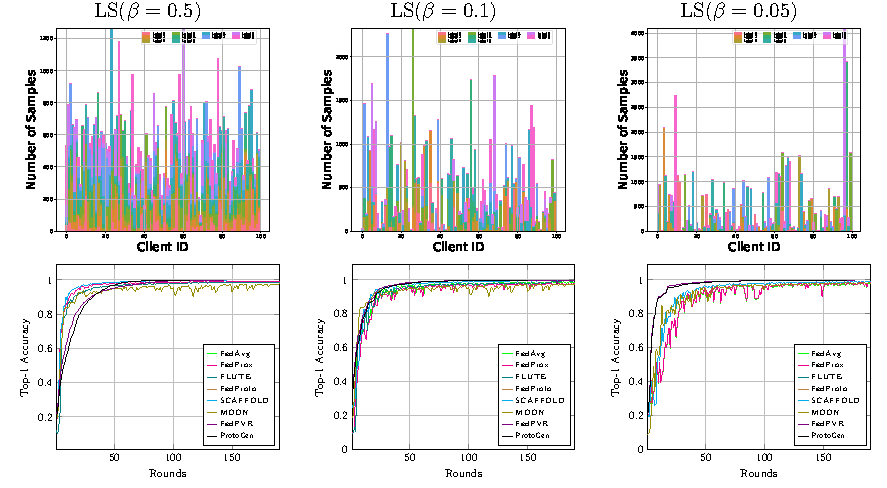
\includegraphics[width=0.5\textwidth]{protogen_mnist_ls_1.pdf}
    \caption{Convergence comparison on MNIST under varying label skew (LS) settings.}

    \label{fig:ds_ls_mnist}
\end{figure}

\begin{figure}
    \centering    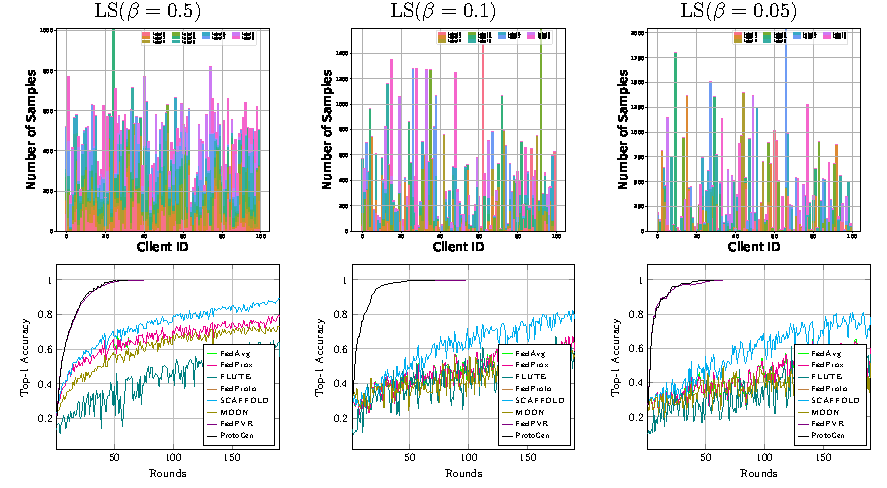
\includegraphics[width=0.5\textwidth]{protogen_cifar_ls_1.pdf}
    \caption{Convergence comparison on CIFAR-10 under varying label skew (LS) settings.}

    \label{fig:ds_ls_cifar}
\end{figure}

\begin{figure}
    \centering    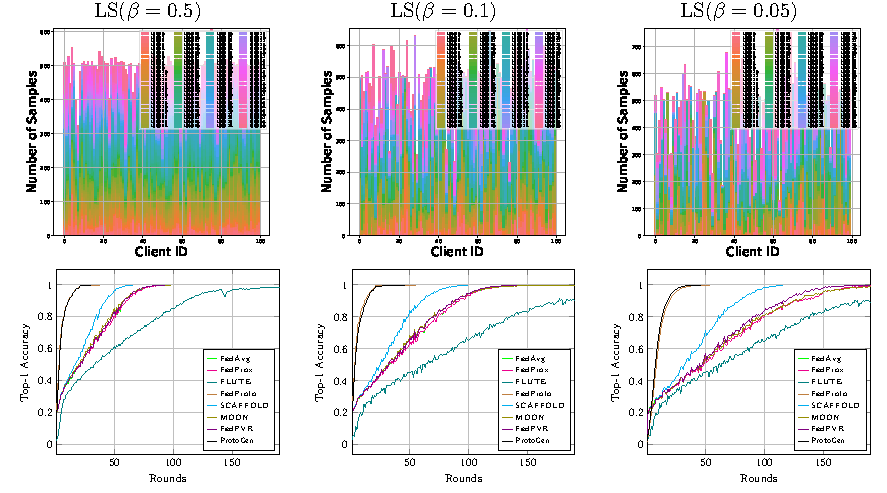
\includegraphics[width=0.5\textwidth]{protogen_cifar100_ls_1.pdf}
    \caption{Convergence comparison on CIFAR-100 under varying label skew (LS) settings.}

    \label{fig:ds_ls_cifar100}
\end{figure}


\begin{figure*}[h!]
\centering
% \renewcommand{\arraystretch}{1.5}
\begin{tabular}{cccc}
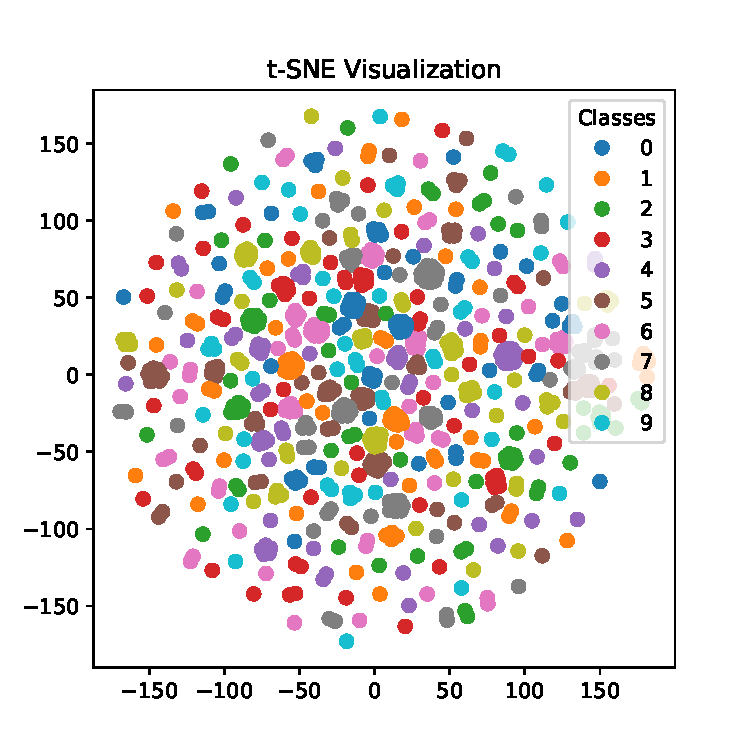
\includegraphics[width=0.23\textwidth]{TSNE/Feature_0.pdf} &
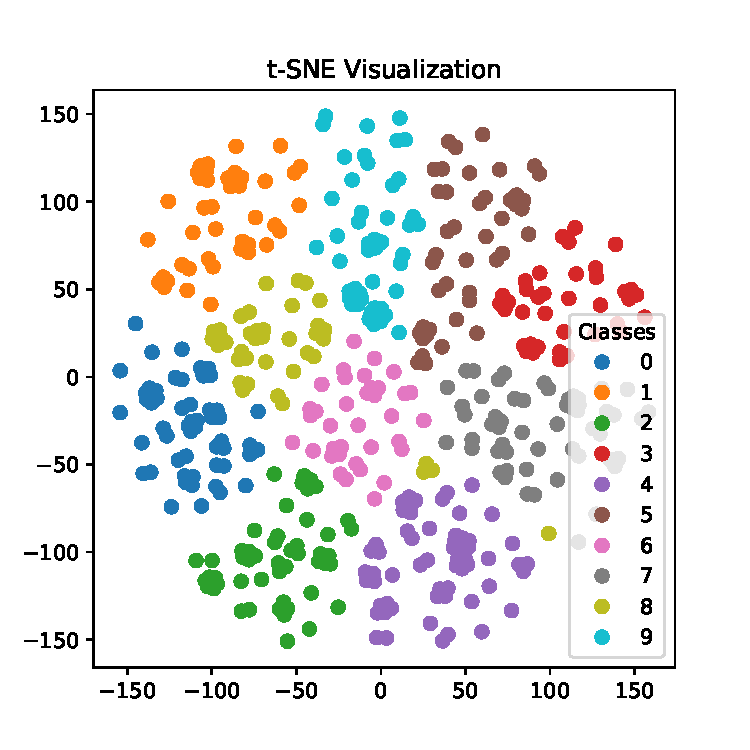
\includegraphics[width=0.23\textwidth]{TSNE/Feature_30.pdf} &
% 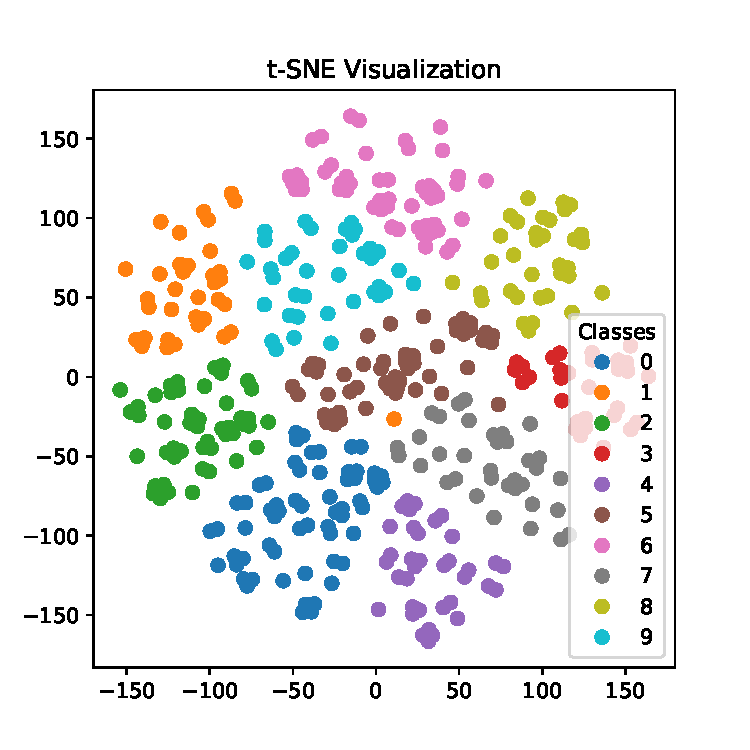
\includegraphics[width=0.25\textwidth]{TSNE/Feature_50.pdf} &
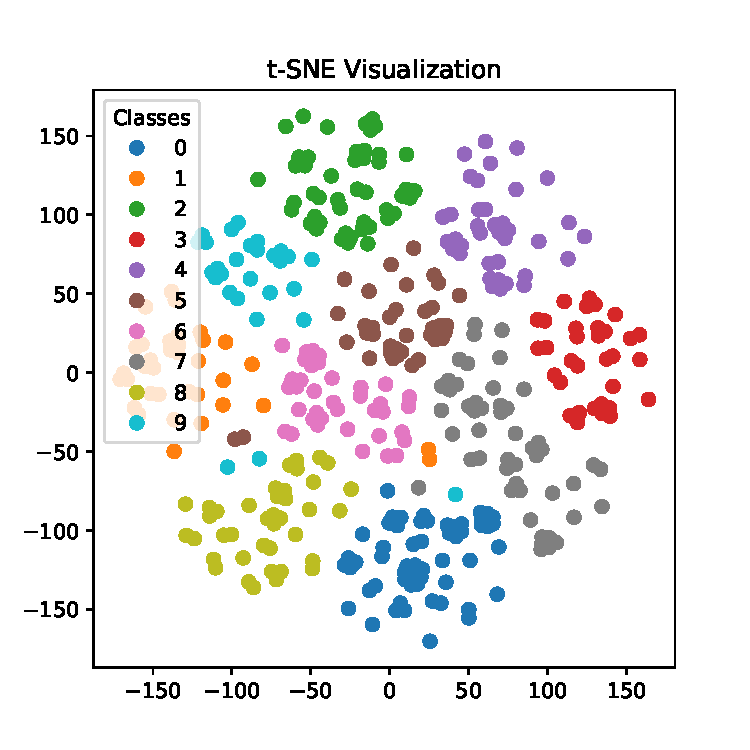
\includegraphics[width=0.23\textwidth]{TSNE/Feature_100.pdf} &
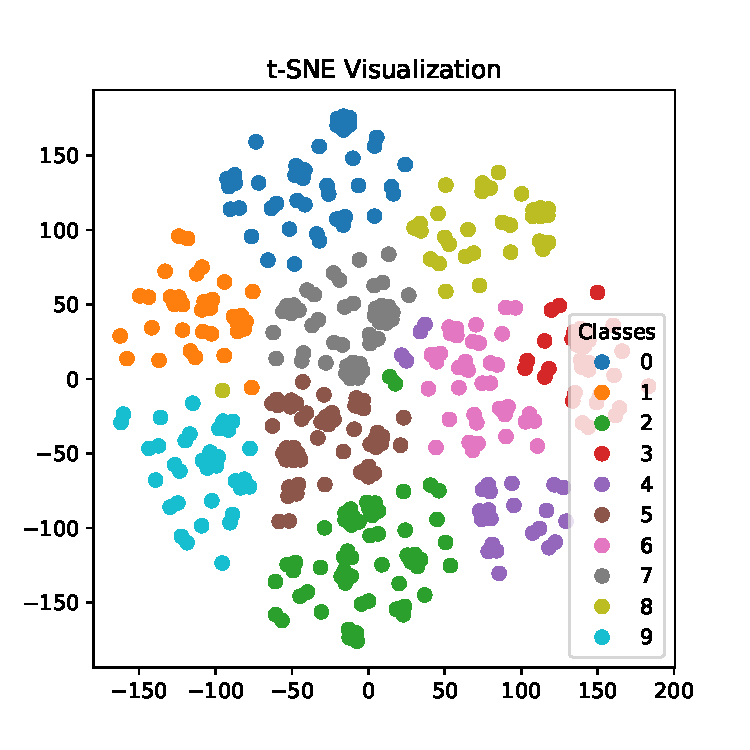
\includegraphics[width=0.23\textwidth]{TSNE/Feature_150.pdf} \\
(a) Round 0 & (b) Round 30 & (c) Round 100 & (d) Round 150
\end{tabular}
\caption{t-SNE visualization of the features generated by client's features generation parameters at different rounds of training. We consider label skew partition with $\beta = 0.5$ for CIFAR-10 dataset.}
\label{fig:t-SNE}
\end{figure*}

\subsection{Visualization of Generated Features}
Figure \ref{fig:t-SNE} presents the t-SNE visualization of features generated by clients' feature generation parameters at different rounds of training. The visualization is based on a label skew partition with $\beta = 0.5$ for the CIFAR-10 dataset.
The result demonstrate that in the beginning of the round the generated features are scattered without clear class boundaries, indicating that the feature generation module has not yet learned meaningful class representations (Figure \ref{fig:t-SNE}(a)). As training progresses to Round 30 (Figure \ref{fig:t-SNE}(b)), the formation of distinct clusters is observed, which suggests that the feature generation module is starting to capture class-specific characteristics.
By Round 100 (Figure \ref{fig:t-SNE}(c)), the clusters become more pronounced and separated, demonstrating improved class discrimination. Finally, at Round 150 (Figure \ref{fig:t-SNE}(d)), we observe a well-defined and tightly clustered class representations, indicating that \textsf{ProtoGen} has successfully learned to generate features that effectively capture the underlying class structure despite the heterogeneous data distribution.


% \begin{table*}[t]
% \centering
% \caption{Privacy Measure Metrics for Various Federated Learning Approaches, here N/A denotes that the privacy measure is not applicable}
% \label{tab:final_privacy_metrics}
% \begin{tabular}{|l|c|c|c|c|}
% \hline
% \textbf{Method}       & \textbf{MIA} ($\downarrow$)  & \textbf{Gradient Leak} ($\downarrow$) & \textbf{Model Inversion} ($\downarrow$) & \textbf{Info Theoretic} ($\downarrow$)\\
% \hline
% FedProto  &  N/A  & N/A            & 1.6876              & N/A \\ \hline
% Scaffold  & 0.4982    & 0.3156            & 1.5937              & 1.5328 \\ \hline
% FedAvg    & 0.4948    & 0.2817            & 1.9949              & 0.1192 \\ \hline
% % FedProx   & 0.4934    & 0.2847            & 1.9364              & 0.1367 \\ \hline
% Elastic    & 0.5088    & 0.3217            & 2.0949              & 0.1282 \\ \hline
% FedFA     & 0.4973    & 0.2719            & 1.9393              & 0.1406 \\ \hline
% \textsf{ProtoGen}     & N/A    & N/A            & 0.3103              & N/A \\ \hline
% \end{tabular}
% \end{table*}

% \subsection{Communication Efficiency}
% Communication costs have always been posed as a challenge in FL, considering several limitations in existing communication channels. Therefore, we also report the amount of data shared between clients and the server per round in Table \ref{tab:baseline_comparison}. It can be seen that the amount of data communicated per round in \textsf{ProtoGen} is much less from all the baselines except FedProto. \todo{add little more depth} 

\subsection{Communication Efficiency}

% Communication costs have always been posed as a challenge in FL, considering several limitations in existing communication channels. Therefore, we also report the amount of data shared between clients and the server per round in Tables \ref{tab:baseline_comparison_ls} and \ref{tab:baseline_comparison_fc}.
Communication efficiency is a critical concern in FL, especially under constrained network conditions and limited bandwidth. To evaluate this, in Tables \ref{tab:baseline_comparison_ls} and \ref{tab:baseline_comparison_fc}, we report the amount of data exchanged between clients and server per round, along with the number of global rounds required to converge. As observed, both \textsf{ProtoGen} and \textsf{ProtoGen}$^+$ consistently outperform the baselines in terms of convergence speed in all heterogeneous settings under consideration.
% Across both data heterogeneity scenarios, \textsf{ProtoGen} consistently outperforms baseline methods in terms of convergence speed (total global rounds to converge). It is observed that \textsf{ProtoGen} and \textsf{ProtoGen}$^+$ converge faster compare to baselines across all the settings. 
While FedProto is converging faster among the baselines, MOON and FLUTE, on the other hand, have slower convergence suggesting the requirement of more communication rounds. Additionally, the results reveal that \textsf{ProtoGen}$^+$ and FedProto have the lowest communication cost per round due to their simple strategy of transmitting lightweight class-wise prototypes, whereas SCAFFOLD has the highest communication cost per round. On the other hand, \textsf{ProtoGen} demonstrates a significant communication efficiency, transmitting substantially less data per round compared to most baselines, including SCAFFOLD, FLUTE, MOON, and FedProx. This efficiency arises from \textsf{ProtoGen}’s design where clients only share compact generative model parameters (decoder) with the server, instead of full model gradients or weights. It is worth to note that, even though \textsf{ProtoGen}$^+$ maintains equal communication cost per round as of FedProto, due to its faster convergence the overall communication cost becomes lower than FedProto.

% Among all baselines, only FedProto has a lower communication cost per round, due to its simple strategy of transmitting lightweight class-wise prototypes. However, FedProto does so at the cost of reduced representational expressiveness and lower overall accuracy, particularly under extreme heterogeneity. In contrast, \textsf{ProtoGen} maintains an overall low communication cost due to faster convergence while achieving significantly better performance by leveraging a lightweight feature generator that captures semantic structure through global prototypes.
% On the other hand, \textsf{ProtoGen}$^+$, maintains equal communication cost per round as FedProto, still remains more efficient than most conventional baselines and offers the best performance in terms of accuracy and convergence speed.




\begin{figure}[t]
    \centering
    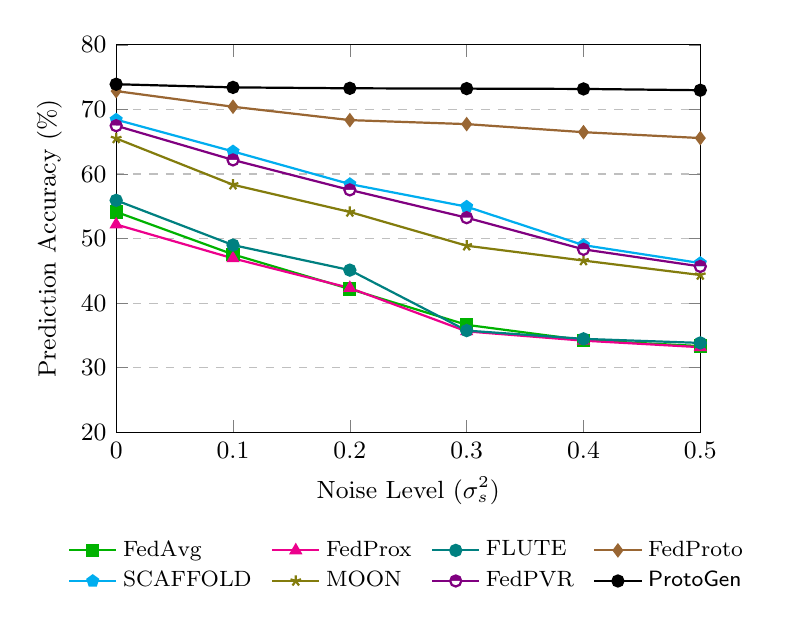
\begin{tikzpicture}
    \begin{axis}[
        width=9cm,
        height=6.5cm,
        xlabel={Noise Level ($\sigma^2_s$)},
        ylabel={Prediction Accuracy (\%)},
        xmin=0, xmax=0.5,
        ymin=20, ymax=80,
        xtick={0.0, 0.1, 0.2, 0.3, 0.4, 0.5},
        ytick={20, 30, 40, 50, 60, 70, 80},
        ymajorgrids=true,
        grid style=dashed,
        tick label style={font=\small},
        label style={font=\small},
        legend style={
            at={(0.5,-0.25)},
            anchor=north,
            font=\footnotesize,
            draw=none,
            fill=none,
            legend cell align=left,
            legend columns=4,
            /tikz/every even column/.style={column sep=5pt}
        },
    ]

    \addplot[green!70!black, mark=square*, thick] coordinates {
        (0.0,54.13)(0.1,47.55)(0.2,42.18)(0.3,36.63)(0.4,34.26)(0.5,33.34)};
    \addlegendentry{FedAvg}

    \addplot[magenta, mark=triangle*, thick] coordinates {
        (0.0,52.18)(0.1,46.93)(0.2,42.34)(0.3,35.62)(0.4,34.18)(0.5,33.17)};
    \addlegendentry{FedProx}

    \addplot[teal, mark=*, thick] coordinates {
        (0.0,55.92)(0.1,48.99)(0.2,45.11)(0.3,35.74)(0.4,34.46)(0.5,33.83)};
    \addlegendentry{FLUTE}

    \addplot[brown!80!black, mark=diamond*, thick] coordinates {
        (0.0,72.85)(0.1,70.42)(0.2,68.35)(0.3,67.73)(0.4,66.48)(0.5,65.57)};
    \addlegendentry{FedProto}

    \addplot[cyan, mark=pentagon*, thick] coordinates {
        (0.0,68.42)(0.1,63.5)(0.2,58.44)(0.3,54.94)(0.4,48.98)(0.5,46.2)};
    \addlegendentry{SCAFFOLD}

    \addplot[olive!90!black, mark=star, thick] coordinates {
        (0.0,65.51)(0.1,58.34)(0.2,54.12)(0.3,48.89)(0.4,46.59)(0.5,44.35)};
    \addlegendentry{MOON}

    \addplot[violet, mark=halfcircle*, thick] coordinates {
        (0.0,67.48)(0.1,62.18)(0.2,57.54)(0.3,53.23)(0.4,48.33)(0.5,45.68)};
    \addlegendentry{FedPVR}

    \addplot[black, mark=otimes*, thick] coordinates {
        (0.0,73.91)(0.1,73.42)(0.2,73.28)(0.3,73.23)(0.4,73.18)(0.5,72.98)};
    \addlegendentry{\textsf{ProtoGen}}

    \end{axis}
    \end{tikzpicture}
    \caption{Prediction accuracy (\%) under varying levels of differential privacy noise ($\sigma_s^2$). The figure compares our approach with baseline methods under different strengths of DP guarantees.}
    % \caption{Prediction accuracy (\%) vs.  differential privacy noise level ($\sigma_s^2$).}
    % \caption{Prediction accuracy (\%) vs.  differential privacy noise level ($\sigma_s^2$). \textsf{ProtoGen} consistently outperforms other FL methods under varying noise levels.}
    % \caption{Impact of differential privacy noise on prediction accuracy. As the privacy noise level ($\sigma_s^2$) increases, most FL methods suffer a significant drop in accuracy. However, \textsf{ProtoGen} demonstrates remarkable robustness, maintaining high predictive performance even under strong noise levels, thus achieving a better trade-off between privacy and utility.}

    \label{fig:privacy}
\end{figure}

\paragraph{Differential Privacy Analysis.} 
To evaluate the robustness of different methods under differential privacy (DP) constraints, we simulate increasing levels of Gaussian noise ($\sigma^2_s$) injected into client data representations. As shown in Figure~\ref{fig:privacy}, most baseline approaches, including FedAvg, FedProx, MOON, and FLUTE, experience a sharp decline in accuracy as the privacy noise increases. This drop is particularly severe for MOON and SCAFFOLD, which rely heavily on precise gradient or representation alignment, making them sensitive to noise perturbations.
In contrast, \textsf{ProtoGen} exhibits a notably stable performance across all privacy levels, maintaining accuracy above 72\% even at the highest noise level ($\sigma^2_s = 0.5$). This resilience is largely attributed to its prototype-based generative mechanism, which aggregates noisy representations into a global class-wise structure, thereby smoothing out local noise through feature-level abstraction. Unlike gradient-sharing methods, \textsf{ProtoGen} avoids transmitting direct model updates, instead relying on semantically meaningful prototypes generated via lightweight decoders.
These results suggest that \textsf{ProtoGen} not only provides strong privacy guarantees due to its minimal sharing and noise-injection strategy, but also preserves predictive accuracy better than other FL approaches under strict DP budgets. Therefore, it achieves a favorable trade-off between privacy preservation and model utility, making it particularly suitable for privacy-sensitive FL applications.


% \subsection{Privacy Preserving}
% Table \ref{tab:final_privacy_metrics} demonstrates \textsf{ProtoGen}'s superior privacy preservation capabilities compared to existing federated learning approaches. Our method achieves the lowest Model Inversion score of 0.3103, significantly outperforming other methods like FedProto (1.6876), SCAFFOLD (1.5937), and FedAvg (1.9949). Moreover, \textsf{ProtoGen} is immune to both Membership Inference Attacks (MIA) and Gradient Leak attacks, as indicated by the N/A symbols, while other methods remain vulnerable to these privacy threats.
% The enhanced privacy protection in \textsf{ProtoGen} stems from our design choice to share only the CVAE model parameters rather than exposing raw features or model gradients. By adding controlled Gaussian noise to the input data before feature extraction, we create a privacy-preserving mechanism that prevents adversaries from reconstructing the original data. This approach effectively maintains the utility of the learned representations for classification tasks while significantly reducing the risk of privacy breaches.
% As shown in Figure \ref{fig:privacy}, we further analyze the relationship between privacy level and model performance by evaluating \textsf{ProtoGen} under different noise levels ($\sigma^2_s$). The results indicate that as the noise level increases from 0.0 to 0.3, there is a gradual decrease in prediction accuracy from approximately 70.05\% to 63.48\%. This demonstrates a clear privacy-utility tradeoff, where stronger privacy guarantees (higher noise levels) come at the cost of slightly reduced model performance. However, even at higher noise levels, \textsf{ProtoGen} maintains reasonable accuracy, outperforming baseline methods in comparable privacy settings.
% Furthermore, the absence of an Info Theoretic score for \textsf{ProtoGen} (indicated by N/A) suggests that those privacy attacks are not applicable to the corresponding method. This comprehensive privacy protection makes \textsf{ProtoGen} particularly suitable for sensitive applications where data privacy is paramount, such as healthcare, finance, and personal mobile applications.


% Better generalization means that samples within the same class cluster in the same area, which can be achieved in a centralized setting, while better personalization means that it is easier to determine to which client the samples belong. It can be seen that samples within the same class but from various clients are close but separable in \textsf{ProtoGen}. This indicates that \textsf{ProtoGen} is more successful in achieving the balance between generalization and personalization, while other methods lack either the generalization or the personalization ability.

\begin{figure}

\begin{tikzpicture}
    \begin{axis}[
            xlabel={Rounds},
            ylabel={Top-1 Accuracy},
            grid=both,
            ymin=0.19,
            width=8.5cm,
            height=6cm,
            xmin=1,
            xmax=190,
            legend style={
            at={(0.80,0.39)},
            anchor=north,
            legend cell align=left,
            legend columns=1,
            font=\scriptsize,
            draw=black, % Remove border around legend
            fill=white, % Remove background color of legend
            inner sep=3pt, % Adjust inner padding of legend box
            legend image post style={scale=0.5}, % Adjust size of legend marker
            },
        ]
\addplot[thick, color=black] table {Tables/cifar_05_sclability/protogen_c200_20.table};
\addplot[thick, color=violet] table {Tables/cifar_05_sclability/protogen_c200_10.table};
\addplot[thick, color=cyan] table {Tables/cifar_05_sclability/protogen_c100_20.table};
\addplot[thick, color=brown] table {Tables/cifar_05_sclability/protogen_c100_10.table};
\addlegendentry {$\sK-200, \sS_t-20$}
\addlegendentry {$\sK-200, \sS_t-10$}
\addlegendentry {$\sK-100, \sS_t-20$}
\addlegendentry {$\sK-100, \sS_t-10$}
\end{axis}
             
\end{tikzpicture}
    % \caption{Scalability Performance of \textsf{ProtoGen} with varying number of total clients ($\sK$) and number of participants per round ($\sS_t$)}
    \caption{Scalability Performance of \textsf{ProtoGen} with varying number of total clients ($\sK$) and number of participants per round ($\sS_t$) on CIFAR-10 under  LS($\beta = 0.5$), using the ResNet-8 model.}
    \label{fig:sclablity}
\end{figure}

\subsection{Scalability of \textsf{ProtoGen}}
To evaluate \textsf{ProtoGen}'s scalability, we conduct experiments on the CIFAR-10 dataset using four distinct configurations that vary both the total client pool size and per-round participation rates. The results in Figure \ref{fig:sclablity} demonstrate \textsf{ProtoGen}'s robust performance across these diverse settings.
With 200 total clients and only 10\% participation per round ($\mathcal{K}$-200, $\mathcal{S}_t$-10), \textsf{ProtoGen} maintains strong performance despite the challenging sparse participation scenario. When further reducing participation to just 5\% ($\mathcal{K}$-200, $\mathcal{S}_t$-10), \textsf{ProtoGen} continues to demonstrate resilience with a slightly reduced convergence trajectory.
For the 100-client configurations, we observe accelerated initial convergence compared to the 200-client settings, attributable to the higher participation rates (20\% and 10\%, respectively). The $\mathcal{K}$-100, $\mathcal{S}_t$-20 setting exhibits particularly impressive performance, suggesting this balanced configuration effectively leverages \textsf{ProtoGen}'s feature generation capabilities.
Across all scenarios, \textsf{ProtoGen} shows consistent improvement as communication rounds progress. This sustained improvement trajectory indicates that \textsf{ProtoGen}'s feature generation approach effectively accumulates knowledge over time, even with limited client participation.
These results underscore \textsf{ProtoGen}'s practical applicability in large-scale federated learning deployments.


\begin{figure}
    \centering
    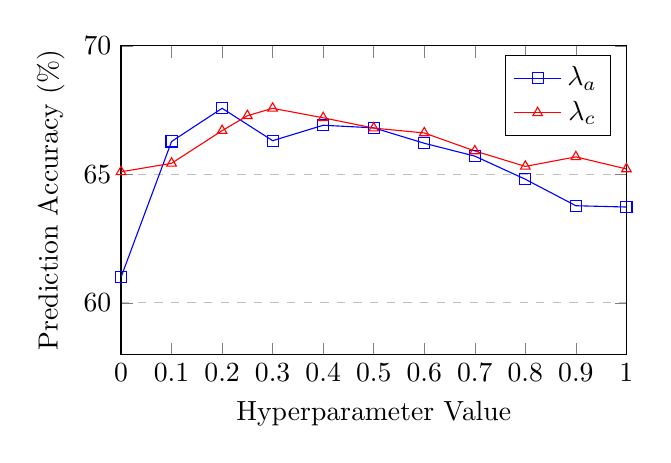
\begin{tikzpicture}
\begin{axis}[
    width=8cm,
    height=5.5cm,
    xlabel={Hyperparameter Value},
    ylabel={Prediction Accuracy (\%)},
    xmin=0.0, 
    xmax=1.0,
    ymin=58, ymax=70,
    xtick={0.0, 0.1, 0.2, 0.3, 0.4, 0.5, 0.6, 0.7, 0.8, 0.9, 1.0},
    legend pos=north east,
    ymajorgrids=true,
    grid style=dashed,
]

\addplot[
    color=blue,
    mark=square,
    ]
    coordinates {
    (0.0,61)(0.1,66.28)(0.2,67.57)(0.3,66.31) (0.4,66.91) (0.5,66.81) (0.6,66.21) (0.7,65.71) (0.8,64.81) (0.9,63.78) (1.0,63.73)
    };
    \addlegendentry{$\lambda_a$}

\addplot[
    color=red,
    mark=triangle,
    ]
    coordinates {
    (0.0,65.1)(0.1,65.43)(0.2,66.7)(0.25,67.28)(0.3,67.57)(0.4,67.2)(0.5,66.8) (0.6,66.61) (0.7,65.91) (0.8,65.31) (0.9,65.68) (1.0,65.21)
    };
    \addlegendentry{$\lambda_c$}

\end{axis}
\end{tikzpicture}

% \caption{Average test accuracy on CIFAR-10 under varying degree of $\lambda_a,\lambda_c$}
% \caption{Average test accuracy on CIFAR-10 with varying values of $\lambda_a$ and $\lambda_c$ under Dirichlet data distribution among 100 clients ($\beta = 0.5$), using the ResNet-8 model.}
\caption{Average test accuracy on CIFAR-10 using the ResNet-8 model under a Dirichlet data distribution among 100 clients ($\beta = 0.5$). Results are reported for varying $\lambda_a$ with fixed $\lambda_c = 0.3$, and varying $\lambda_c$ with fixed $\lambda_a = 0.2$.}

\label{fig:abltn_study}
\end{figure}

\subsection{Ablation Study}
To understand the contribution of different components in our proposed \textsf{ProtoGen} framework, we conduct an ablation study by varying the hyper-parameters $\lambda_a$ and $\lambda_c$, which control the strength of feature alignment and classifier regularization, respectively as mentioned in Equation \ref{eq:combined_objective}. As shown in Figure \ref{fig:abltn_study}, we observe that both hyper-parameters significantly impact the model's performance on the CIFAR-10 dataset.
For $\lambda_a$, which controls the alignment between local features and global prototypes, we observe that the accuracy initially increases as $\lambda_a$ increases from 0.01 to 0.5, reaching a peak of 66.89\% at $\lambda_a = 0.2$. However, beyond this point, the accuracy decreases significantly, dropping to 65.31\% at $\lambda_a = 0.5$. This suggests that while some degree of feature alignment is beneficial for addressing heterogeneity, excessive alignment can be detrimental, potentially forcing the model to discard client-specific information that is valuable for local predictions.
Similarly, for $\lambda_c$, which regulates the classifier training on generated features, we observe a peak accuracy of 66.89\% at $\lambda_c = 0.3$. The accuracy curve for $\lambda_c$ is more gradual, with a slower decline after the peak compared to $\lambda_a$. This indicates that the classifier regularization component is more robust to hyperparameter variations, providing consistent benefits across a wider range of values.
These results highlight the importance of carefully balancing the different components of \textsf{ProtoGen} to achieve optimal performance. The ablation study confirms that both feature alignment and classifier regularization contribute significantly to \textsf{ProtoGen}'s effectiveness in heterogeneous federated learning environments, but their relative importance and optimal settings depend on the specific dataset and heterogeneity conditions.



\section{Conclusion}
\label{sec:conclusion}
This paper presents a novel FL approach, aiming to mitigate the effect of data heterogeneity while improving communication efficiency and privacy preservation. By leveraging a feature generation module, \textsf{ProtoGen} enables clients to share only lightweight feature generation parameters with the server, rather than full local model parameters. This approach not only helps to mitigates privacy risks but also reduces communication overhead. To address the challenges of data heterogeneity, \textsf{ProtoGen} trains local models by aligning their hidden features with global feature prototypes, ensuring consistent intra-class representations while enhancing inter-class distinctions. Additionally, a privacy-preserving generative model is employed to allow clients to capture a more generalized local pattern from the dataset helping the server to construct a unbiased global representation. 
%%\todoa{To further reduce communication cost we also introduce \textsf{ProtoGen}$^+$ (a communication-efficient variant of \textsf{ProtoGen}) that allows clients to share only local class-wise prototypes with the server and server aggregates them to construct global prototypes.} 
Experimental results demonstrates a significant performance improvement by an average of 4.76\% over state-of-the-art FL methods and 2.61\% with respect to the second best performer in terms of accuracy. This highlights \textsf{ProtoGen}’s ability to enhance the performance of underrepresented classes in clients, leading to a more balanced and equitable learning outcome. Furthermore, \textsf{ProtoGen} exhibits faster convergence rates with reduced communication cost compared to existing methods, maintaining its performance advantages even in extreme heterogeneous settings. 
%While \textsf{ProtoGen}$^+$ (a communication-efficient variant of \textsf{ProtoGen}) that achieves comparable performance as of \textsf{ProtoGen}, it significantly reduces communication overhead by an average of 84.44\% compared to \textsf{ProtoGen}.
As an interesting note, we find \textsf{ProtoGen}$^+$ (a communication-efficient variant of \textsf{ProtoGen}) not only achieves performance comparable to \textsf{ProtoGen}, but also reduces communication overhead by an average of 84.44\% compared to \textsf{ProtoGen}. However, this comes at the cost of  some compromise in privacy.

\bibliographystyle{ieeetr}
\bibliography{reference}


% \section{Conclusion}
% \label{sec:conclusion}

% \bibliography{iclr2025_conference}
% \bibliographystyle{iclr2025_conference}

% \appendix
% \section{Appendix}
% You may include other additional sections here.


\end{document}
